\status{done}
\chapter{muEDM positron tracker}
\label{ch:muEDM:tracker}
\begin{refsection}
{\itshape This chapter is an in-depth study on the development of the scintillating fiber part of the muEDM positron tracker. 
We will skip some preliminary studies and we will start with the description of the positron tracker which was included in the proposal of the experiment submitted to PSI at the end of 2022. We will move to the simulations done after that and the current design of this detector.}

\status{done}
\section{Tracking $\Ae$ in muEDM}
    As already introduced in Ch.~\ref{ch:muEDM}, the muEDM experiment is based on the \textit{frozen spin} technique.
    For this purpose, it is cardinal to stop the muon in the right orbit. 
    After the muon has been stored, the careful calibration of the radial electric field will then change the $(g-2)$ precession, bringing it eventually to 0.
    At this point, the direction of the positron emission will be the relevant variable for the EDM search.
    These three steps require a way to track the outgoing $\Ae$.
    Developing such a tracker in the muEDM environment is the challenge to which this chapter is dedicated.\\

    \noindent
    We will start by presenting the detector included in the proposal of 2022 and then the version obtained in 2023 refining the original design.
    The original detector design was developed to be complemented with silicon devices.
    By the end of 2023, the requirement for this detector changed, with the delay of the Pixel sub-detector. 
    Some studies on a radial solution will close the chapter.
    
\status{done}
\section{Design in the 2022 proposal}
\label{sec:muEDM:proposal}
    The kinematics of the $e^+$ coming from the decay was already discussed in a Sec.~\ref{sec:muEDM:sensitivity}.
    From preliminary results, the resolutions required for the different studies are the following:
    \begin{outline}
        \1 Momentum resolution: around a few MeV/c. 
        This is necessary for selection cuts on positrons with the desired asymmetry, which is momentum dependent, as discussed in Sec~\ref{sec:muEDM:sensitivity}.
        \1 Position resolution: around \SI{1}{mm}. This seems to be the necessary resolution for track fitting with the required uncertainties on the emission direction. 
        This result was achieved by geometric means, assuming that reliable timing information is not available. 
        \1 Timing resolution: less than \SI{1}{ns}. The \SI{28}{MeV/c} positron travels at \textit{c}, meaning that in the expected magnetic field a complete rotation takes $\gtrsim$ \SI{0.6}{ns} imposing this limit. 
    \end{outline}
    \noindent
    To accomplish these requirements, the idea was to implement a two sub-system tracker: a positron tracker based on scintillating fibers of $250\divisionsymbol\SI{1000}{\micro\meter}$ size coupled to silicon photomultipliers~(SiPM) plus a tracker based on the silicon Pixel technology, developed by the UK part of the collaboration.  
    The scintillating fiber part of the detector allows for a fast, versatile, modular, and low-cost detector technology that is operational in magnetic fields and vacuum, the environment in which the muEDM measurement takes place.
    
    \begin{figure}
        \centering
        \subfloat[Sketch of the SciFi conceptual design. The outer part is made of eight ribbons, with the fibers oriented longitudinally.]{\hspace{0.075\columnwidth}
        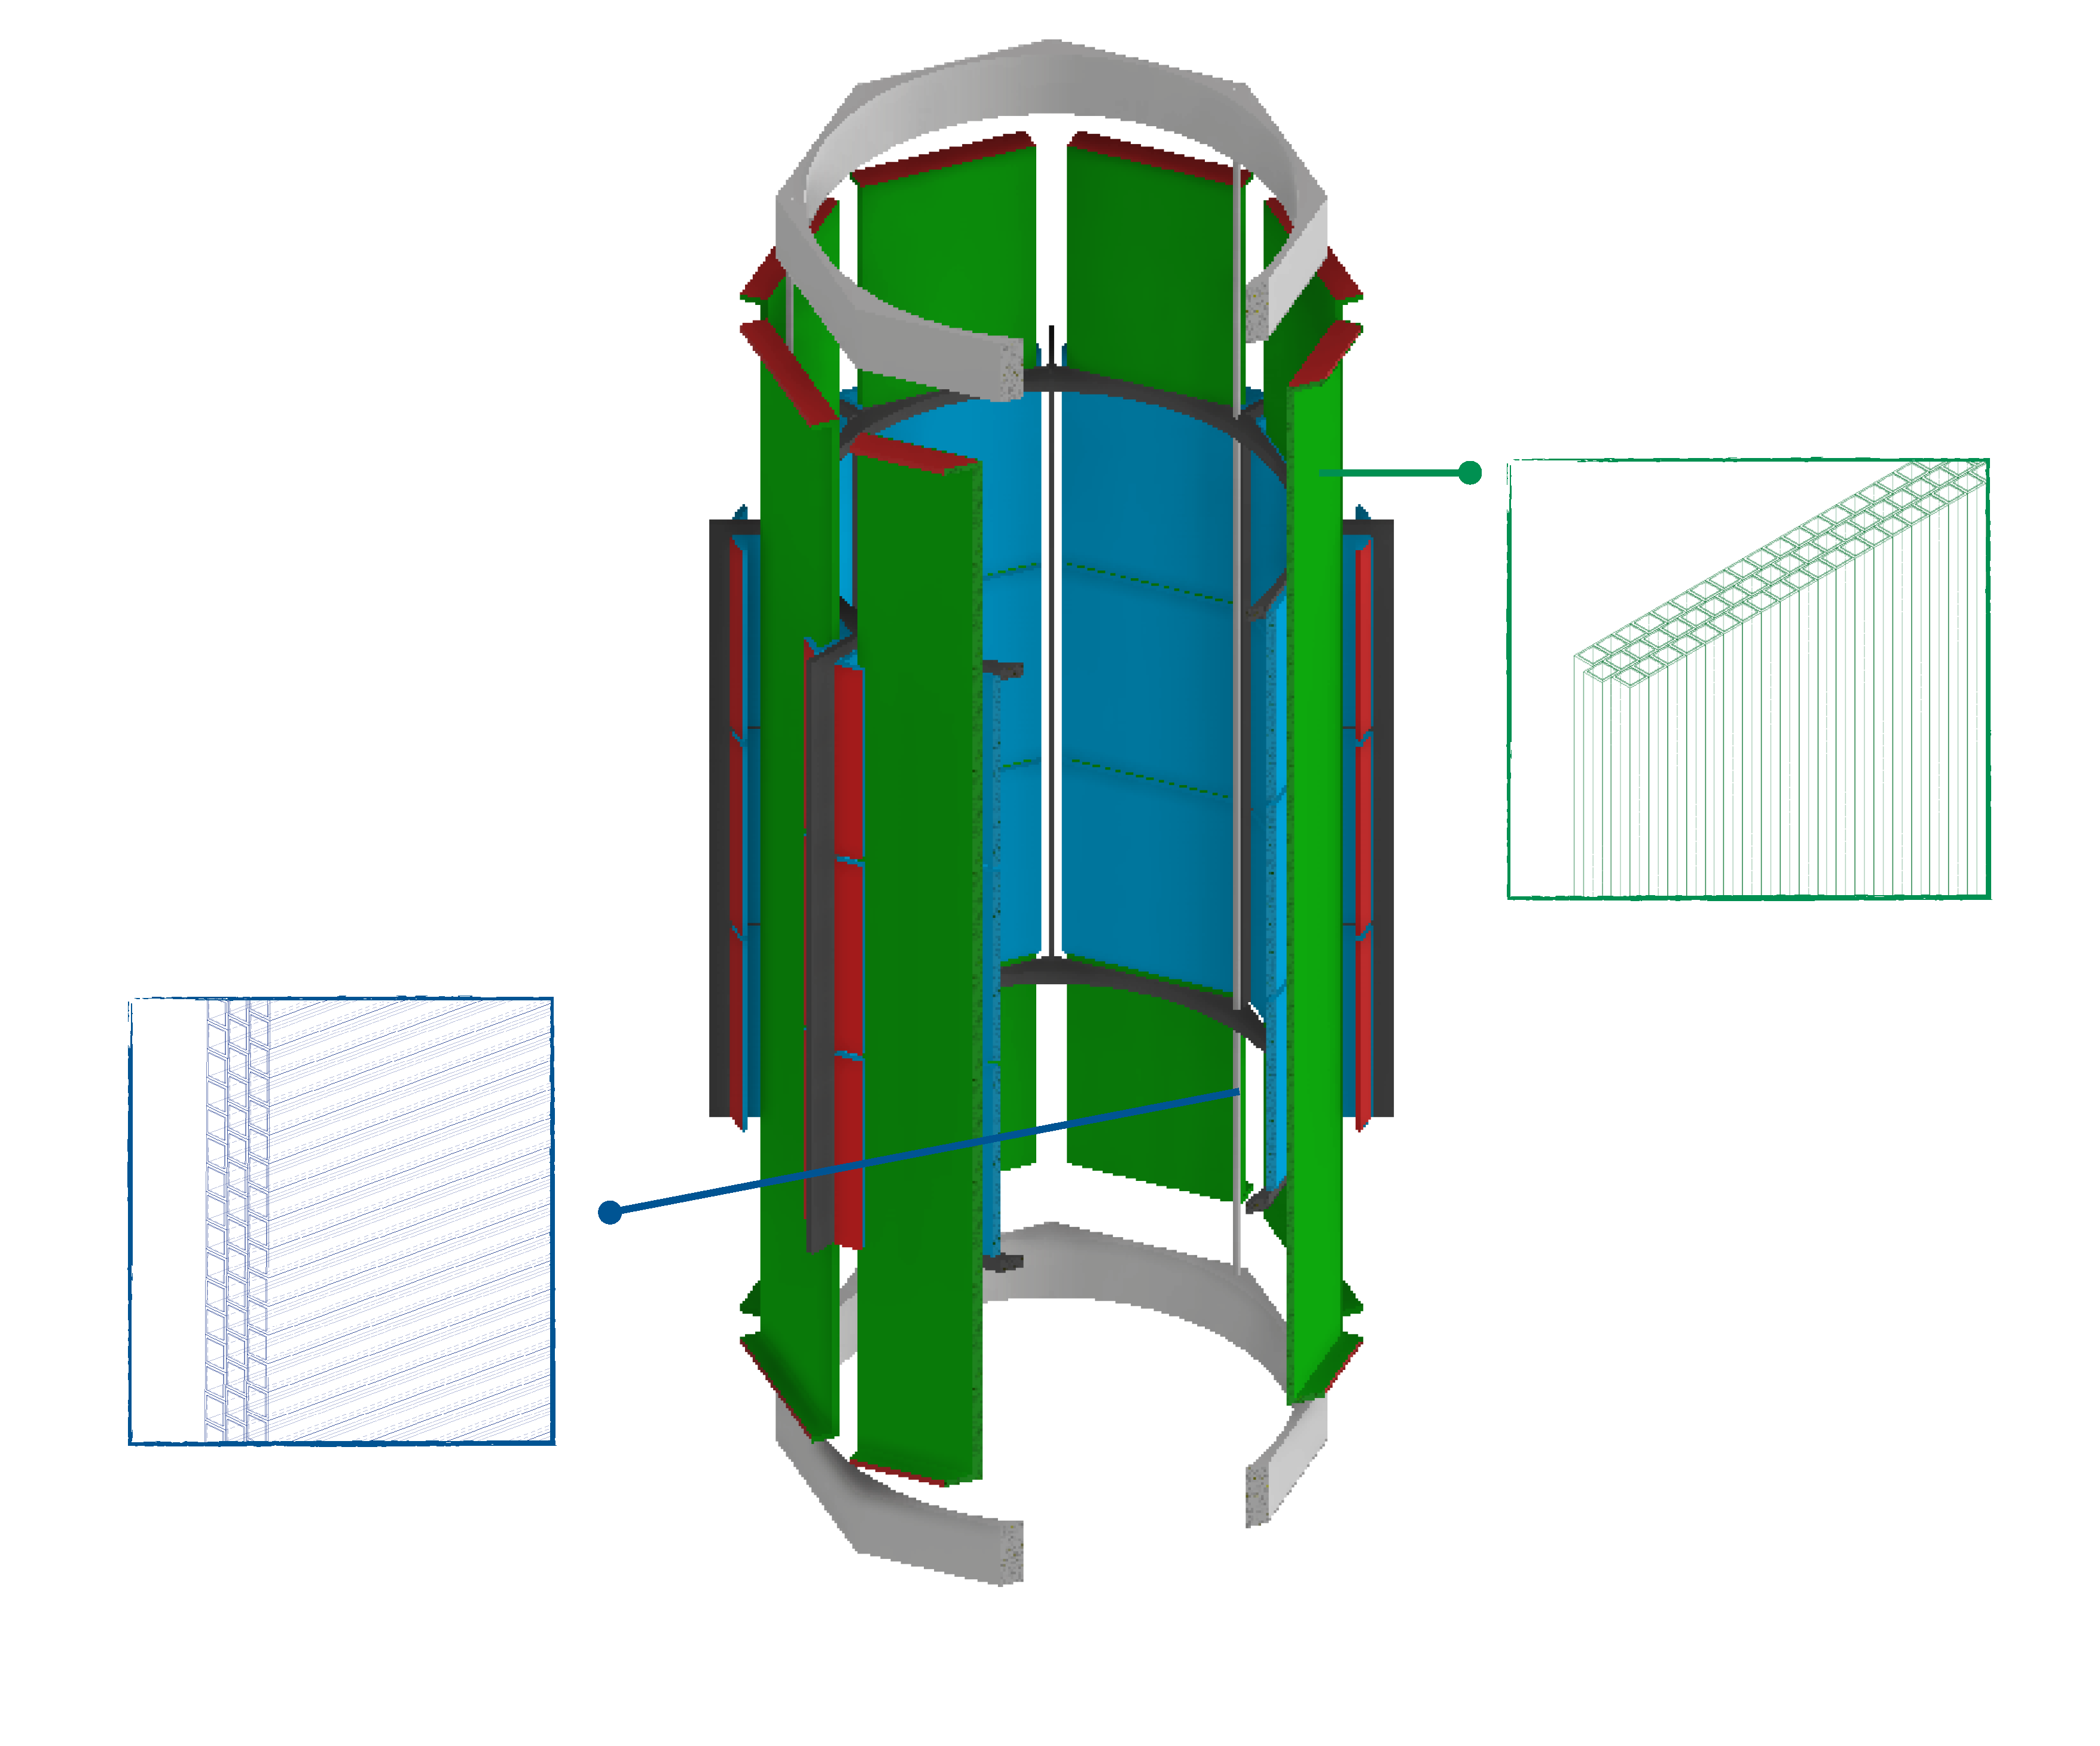
\includegraphics[width=0.55\columnwidth]{Figures/muEDM/Tracker/Assembly_muEDM_SciFi.png}
        \label{fig:SciFi_ConceptualDesign:outer}}
        \hfill
        \subfloat[The inner part is made up of three barrels of scintillating fiber ribbons. Each barrel constitutes eight ribbons, with the fibers oriented transversely.]{
        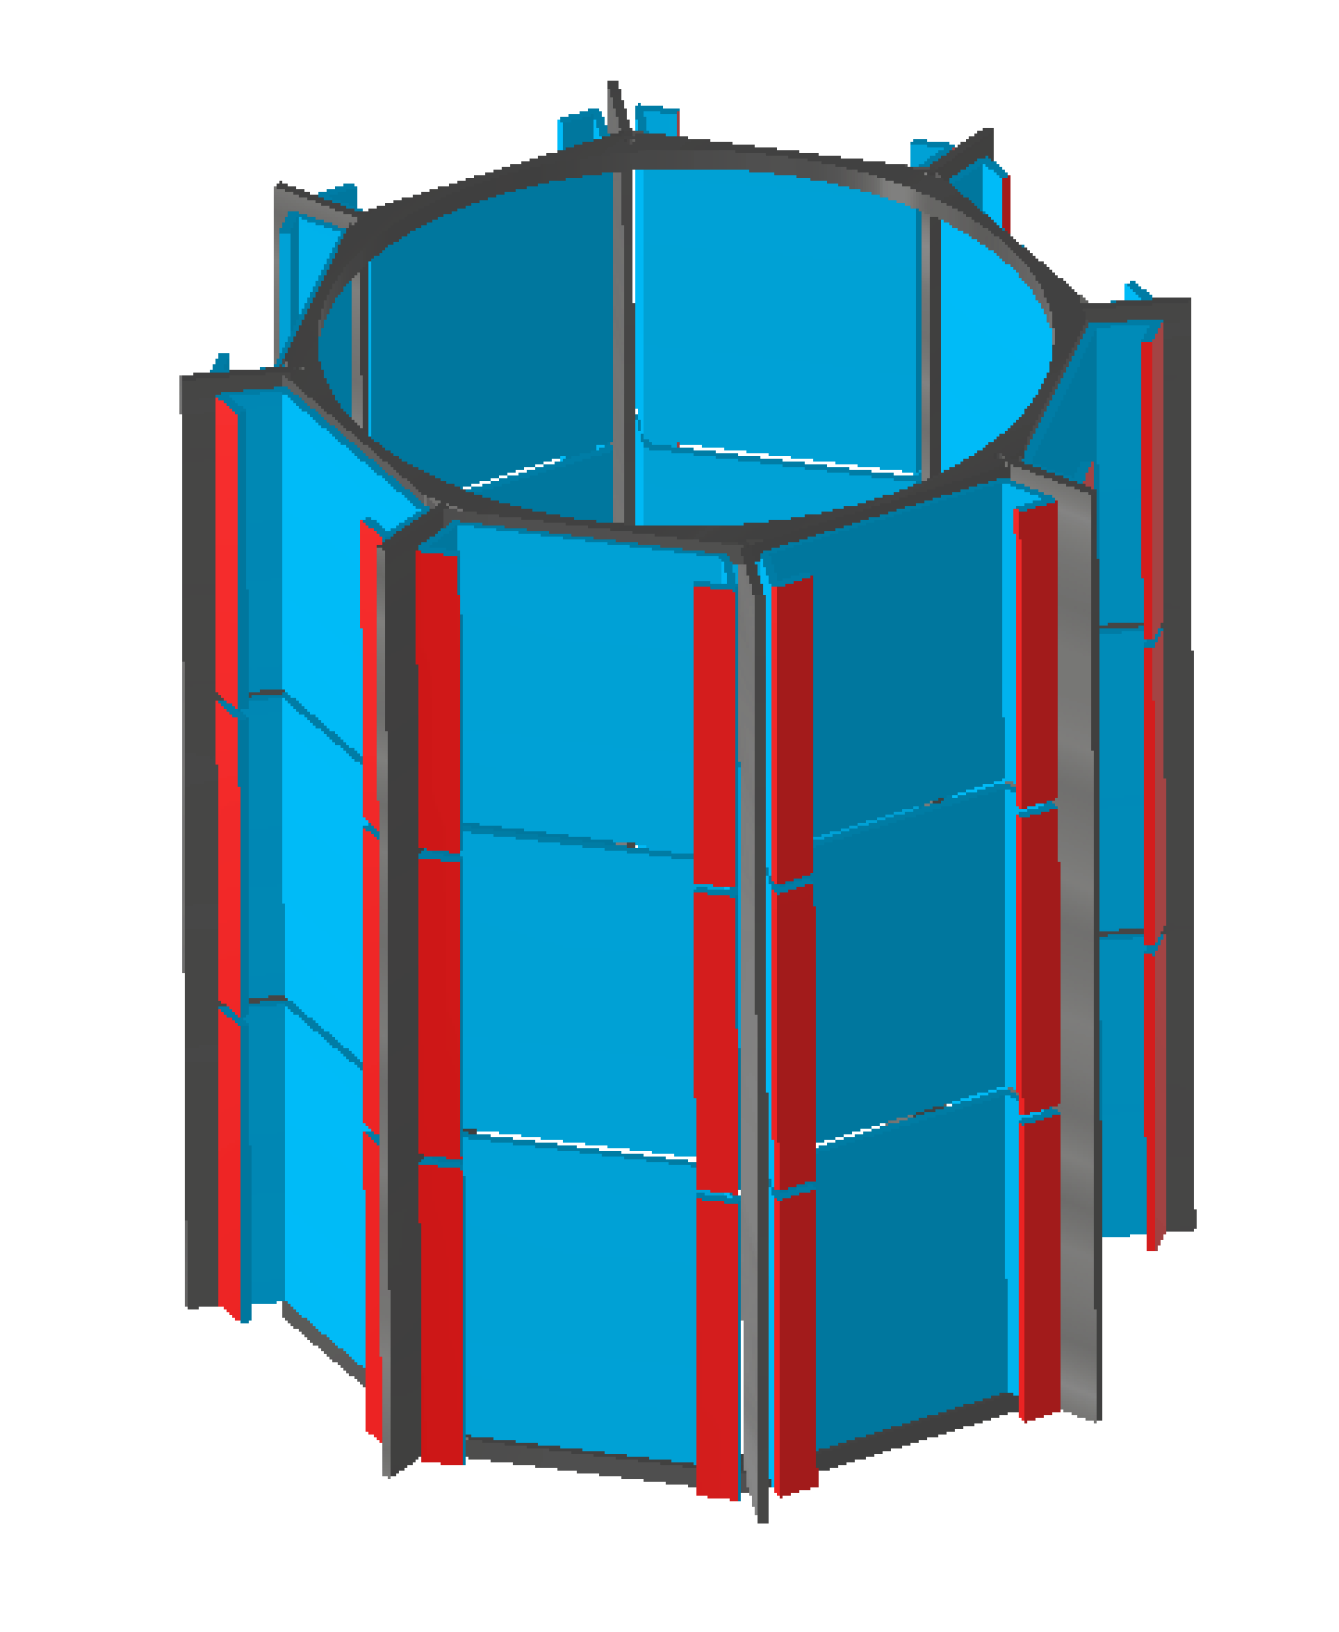
\includegraphics[width=0.25\columnwidth]{Figures/muEDM/Tracker/Assembly_InnerCup.png}        \label{fig:SciFi_ConceptualDesign:inner}
        \hspace{0.075\columnwidth}}
        \hfill
        \subfloat[Left: Sketch of the layout of the fibers inside a SciFi ribbon. Right: A sketch of a fiber that comprises a \textit{core} and two \textit{claddings} of PMMA\@.]{
        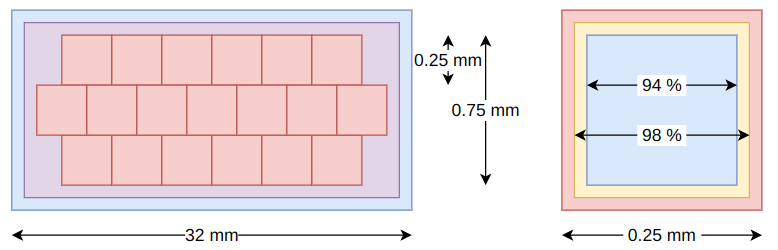
\includegraphics[width=0.5\textwidth]{Figures/muEDM/Tracker/SciFi.png} \label{fig:SciFi_ConceptualDesign:fibers}	}
        \caption[muEDM Tracker: CAD design and SciFi ribbon]{In (a) and (b) the CAD view of the detector design while in (c) the details on the ribbon structure and the fiber \textit{cladding}.}
    \label{fig:SciFi_ConceptualDesign}
    \end{figure}

    \status{done}
    \subsection{The SciFi detector}
        The SciFi detector is designed to provide excellent tracking capacities for minimum-ionizing particles with a detector thickness below \SI{0.4}{\%}, a timing resolution better than \SI{1}{ns}, and a spatial resolution of \SI{1}{mm}, or better.
        Fig.~\ref{fig:SciFi_ConceptualDesign} shows the first conceptual design of the detector. 
        The tracker would be a compact detector made of several \textit{ribbons} of \SI{250}{\micro m} scintillating fibers arranged in an inner~(transverse) and an outer~(longitudinal) detector.
        The inner detector would made of a minimum of three barrels, extendable to five, of scintillating fiber ribbons. Each barrel made of eight ribbons, with the fibers oriented transversely. 
        This is the SciFi transverse detector, as shown in Fig.~\ref{fig:SciFi_ConceptualDesign:inner}, providing the necessary longitudinal resolution (up/down) to measure the EDM signal. 
        In this detector, the fiber ribbons are polygonally shaped as shown by the blue elements in the figure. The red elements represent the photosensors. 
        The optional outer detector is made of eight ribbons, with the fibers oriented longitudinally. Here, the ribbons have a parallelepipedal shape (green elements) with photosensors at both ends (red elements), as shown in Fig.~\ref{fig:SciFi_ConceptualDesign:outer}. \\
        Each ribbon has three layers of fibers, and these three layers are glued together in a staggered way, as sketched in Fig.~\ref{fig:SciFi_ConceptualDesign:fibers}. Each layer is made up of 128 \SI{250}{\micro m} square or round multiclad fibers, meaning a layer has a width of approximately \SI{32}{mm}.
        Each ribbon is read out at both ends by silicon photomultiplier (SiPM) arrays. 
        Double-readout of each ribbon is essential for matching the experiment requirements.
        The amount of energy deposited in such a thin fiber by a MIP is small ($\mathcal{O}(\SI{35}{keV})$) and, given the size of the detector, the relative light reaching the photosensor turns out to be equal to a few photons/fiber. 
        To successfully collect these few photons with maximum efficiency and high dark noise rejection factor, a double readout scheme is foreseen, as well as extreme care in the coupling of the fibers to the photosensors.

    \status{done}
    \subsection{Scintillating fibers prototype}
    \label{sec:SciFi_prototype}
        A prototype to mimic the behavior of a fiber ribbon was built and tested.     
        It consists of 32 squared, \SI{250}{\micro m} thin multiclad BCF-12 fibers manufactured by Saint-Gobain and it is shown in Fig.~\ref{fig:LargePrototype}. 
        The fibers were assembled to make four fiber layers; the first one was used as a trigger, and the others, staggered by half a fiber, were used to mimic the detector. 
        Each fiber was coated by physical vapor deposition with $\sim \SI{100}{nm}$ of aluminum along its whole length, with the aluminum acting as an optical insulator.
        The fiber ends were fixed on two plexiglass end plates, which were polished with a diamond cutting blade and fixed to an aluminum support structure. 
        Each fiber end was coupled with BC630 optical grease to a Hamamatsu 13360-1350CS SiPM (active area $1.3\times1.3$~mm$^{2}$, pixel size \SI{50}{\micro m}, PDE 40\thinspace\%~\cite{Stoykov2012NIMA}), resulting in 64 channels. 
        All SiPMs were biased at the same bias voltage ($\approx \SI{55}{V}$). 
        The signal was passed through a minicircuit amplifier, working with a typical gain of \SI{40}{dB}, and finally digitized with DRS V5 evaluation boards \cite{Ritt2010NIMA,Galli2014JINST} at a sampling speed of 5 GSPS.
        To emulate the situation in which the fiber tracker is read out column-wise by SiPM arrays (see Fig.~\ref{fig:sipmarray:sketch}), rather than reading out every fiber individually, the information from fibers of three consecutive layers was combined at the software level, as shown in Fig.~\ref{fig:sipmarray:fibercombination}.\\
        
        \begin{figure}
            \centering
            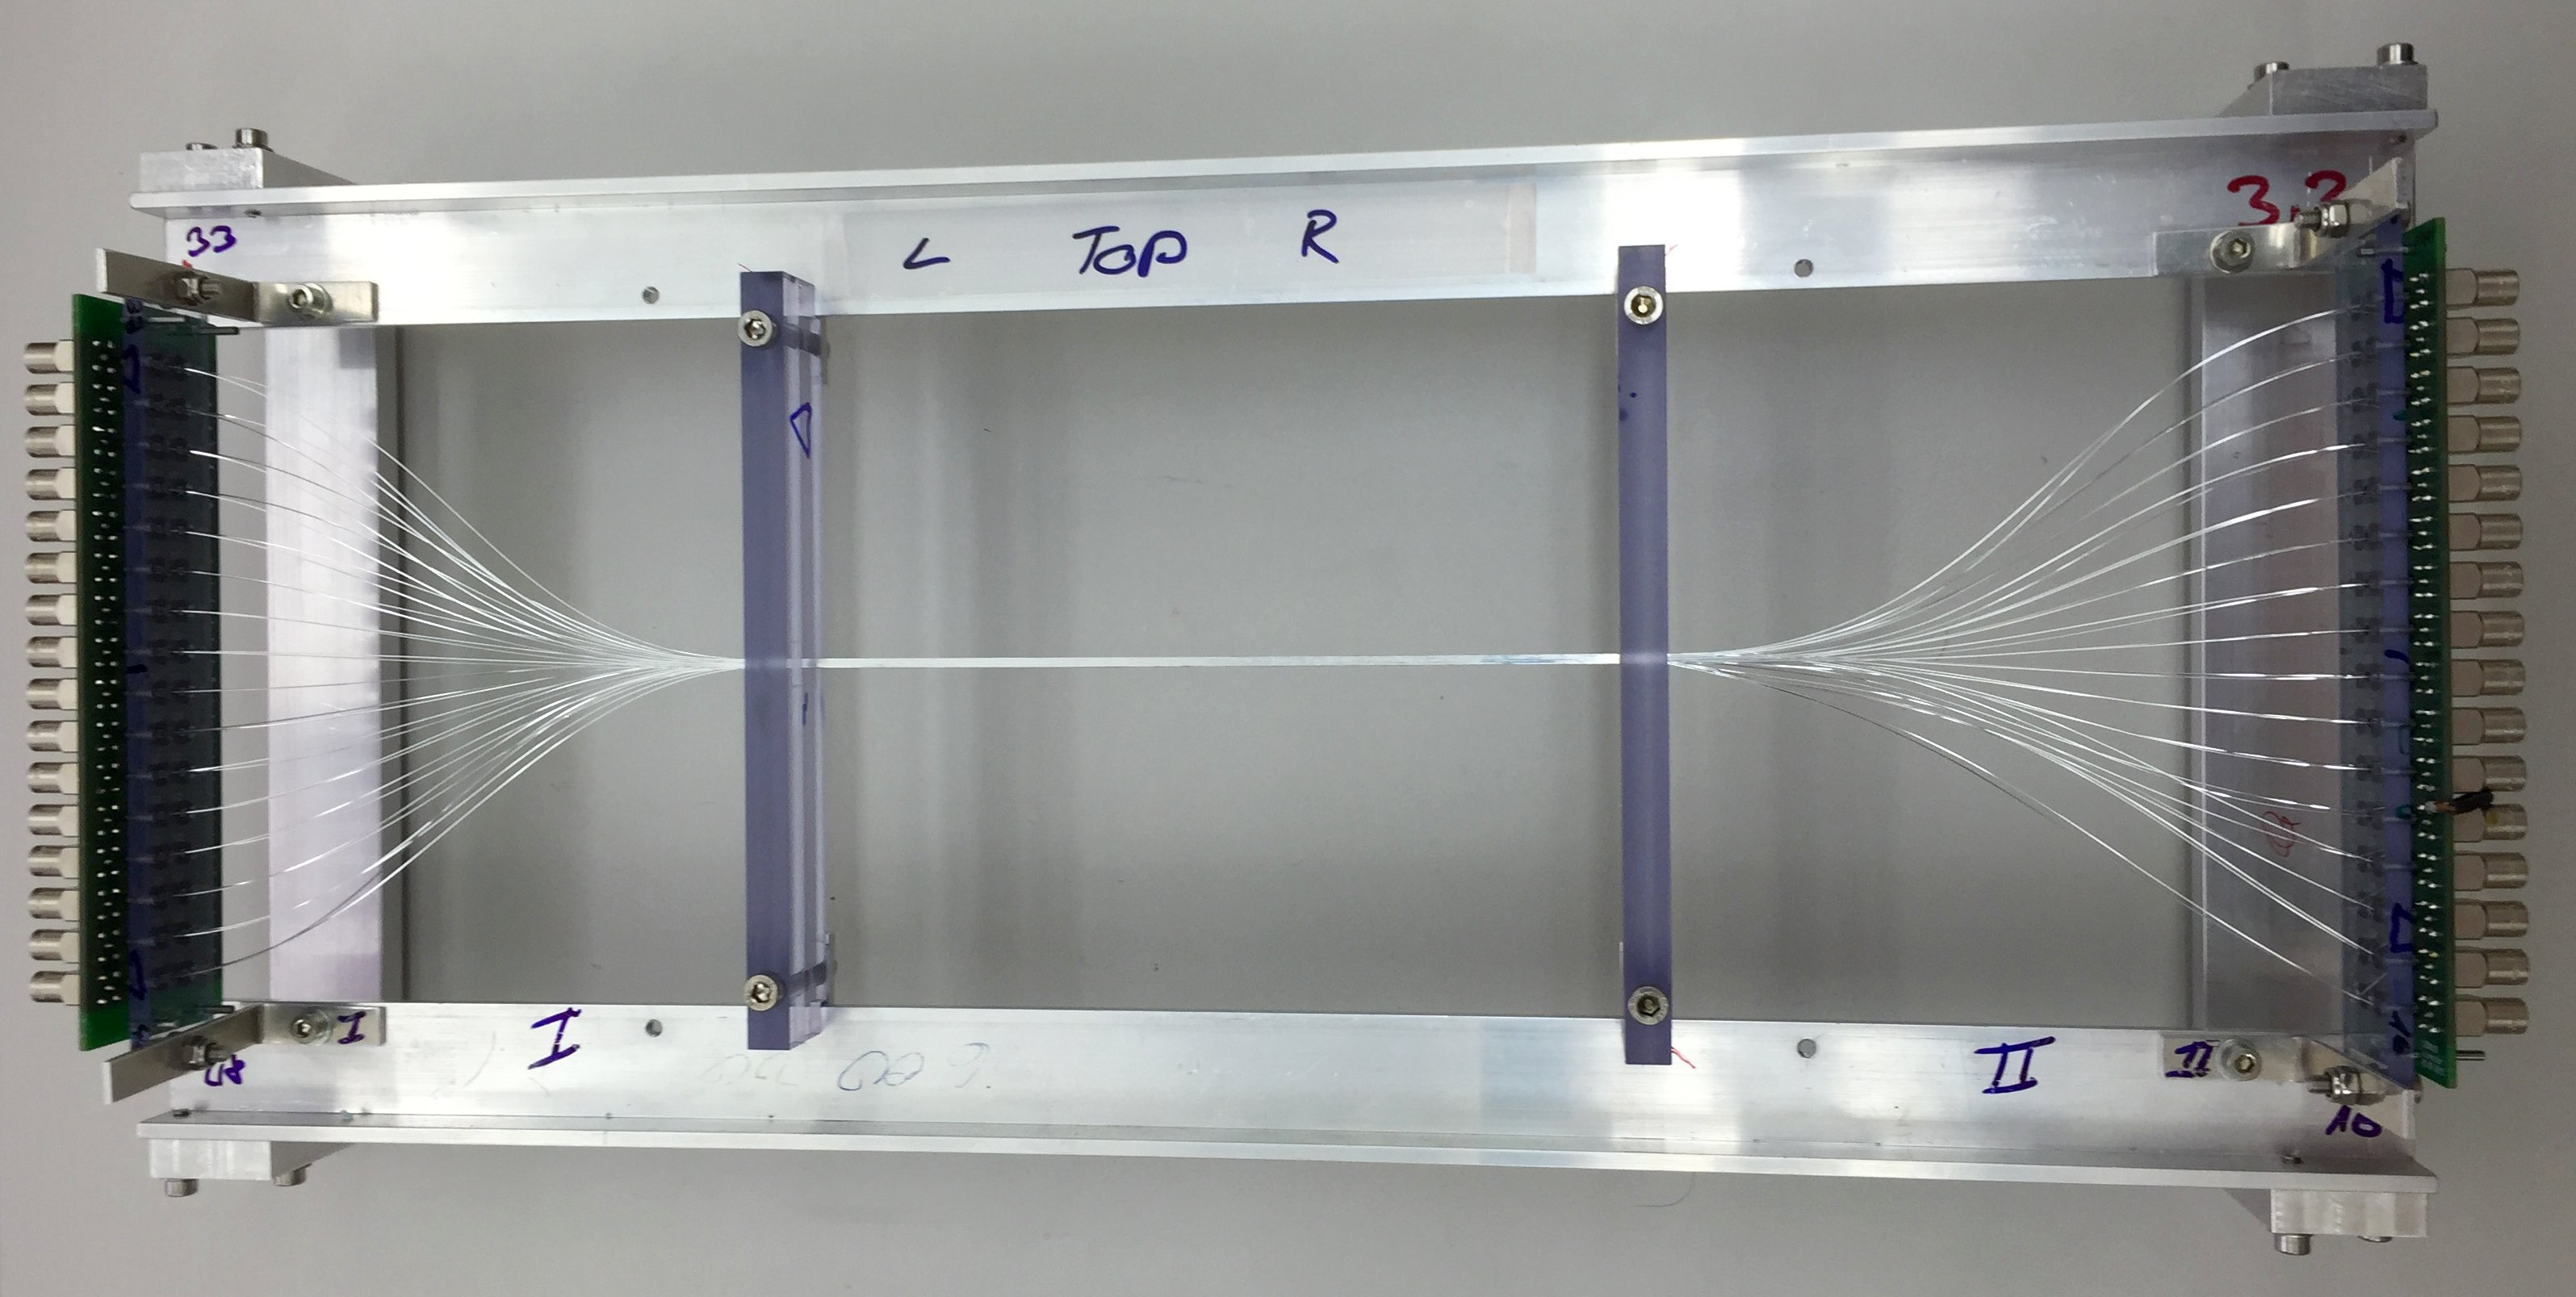
\includegraphics[ width=0.8\textwidth]{Figures/muEDM/prototype/largeprototype.jpg}	
            \caption[SciFi prototype: picture]{The fibers prototype, made of 32~squared, multiclad BCF-12 fibers of \SI{250}{\micro m} thickness. Each fiber is coated with $\sim\SI{100}{nm}$ of aluminum and read out by a SiPM at each end.}
            \label{fig:LargePrototype}
        \end{figure}
             
        \begin{figure}
            \centering
            \subfloat[]{
            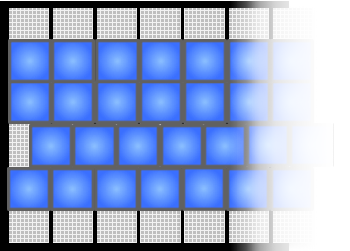
\includegraphics[height=3cm]{Figures/muEDM/prototype/sipmarray.png}
            \label{fig:sipmarray:sketch}} 
            \hspace{0.2\columnwidth}
            \subfloat[]{
            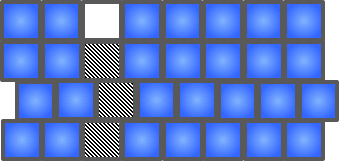
\includegraphics[height=3cm]{Figures/muEDM/prototype/fiberscombined_scheme.png}
            \label{fig:sipmarray:fibercombination}}
            \caption[SciFi prototype: fiber layers]{Illustration of a column-wise readout of fiber tracker using SiPM arrays, rather than reading out every fiber individually. Fiber tracker~(blue) coupled to a SiPM array~(gray/b). Emulation of the column-wise read-out by SiPM arrays, combining offline the SiPM read out~(b).}
            \label{fig:sipmarray}
        \end{figure}

        \noindent
        The prototype was studied in both the laboratory with a $^{90}$Sr source (electrons with endpoint energy \SI{2.28}{MeV}) and at PSI's $\pi$M1 beam line. 
        Unless otherwise stated, the following results refer to measurements at the $\pi$M1 beamline when selecting minimum ionizing positrons and irradiating the fibers at approximately half the fiber length, perpendicularly to their central axes. 
        The $\pi$M1 beam was tuned to positive polarity and to a momentum of \SI{115}{MeV/c}.

        \subsubsection{Results}
        The prototype showed a uniform response (variations between fibers $\lesssim10$\thinspace\%, variations in time and different trigger conditions $\leq 5$\thinspace\%) with the average number of photoelectrons (phe) being $4.6\pm0.3$ (stat) for the AND and $3.7\pm0.3$ (stat) for the OR configuration at a threshold of 0.5~phe, consistent with the expectations. A typical light spectrum is shown in Fig.~\ref{fig:ChargeSpectrumAND}.

        \noindent
        The detection efficiency for both individual and multiple fibers combined was evaluated by using the first fiber layer (and, where appropriate, also preceding / successive fibers) as a trigger. The measured MIP detection efficiency for the different logic configurations, thresholds, and layer numbers are summarized in Table~\ref{tab:DetectionEff}.
        The time resolution on the mean time for a single fiber was determined considering the distribution $T_{single} = (t_{1}-t_{2})/2$, where $t_{1}$ and $t_{2}$ denote the time extracted from the SiPM at the left and right ends of the fiber, respectively. A typical distribution measured for a single fiber is shown in Fig.~\ref{fig:TimingSingleFibre}.

        \begin{figure}
            \centering
            \subfloat[Typical light spectrum (th. 0.5~phe) measured by a single \SI{250}{\micro m} square multiclad fiber ($\approx \SI{50}{cm}$ length).]{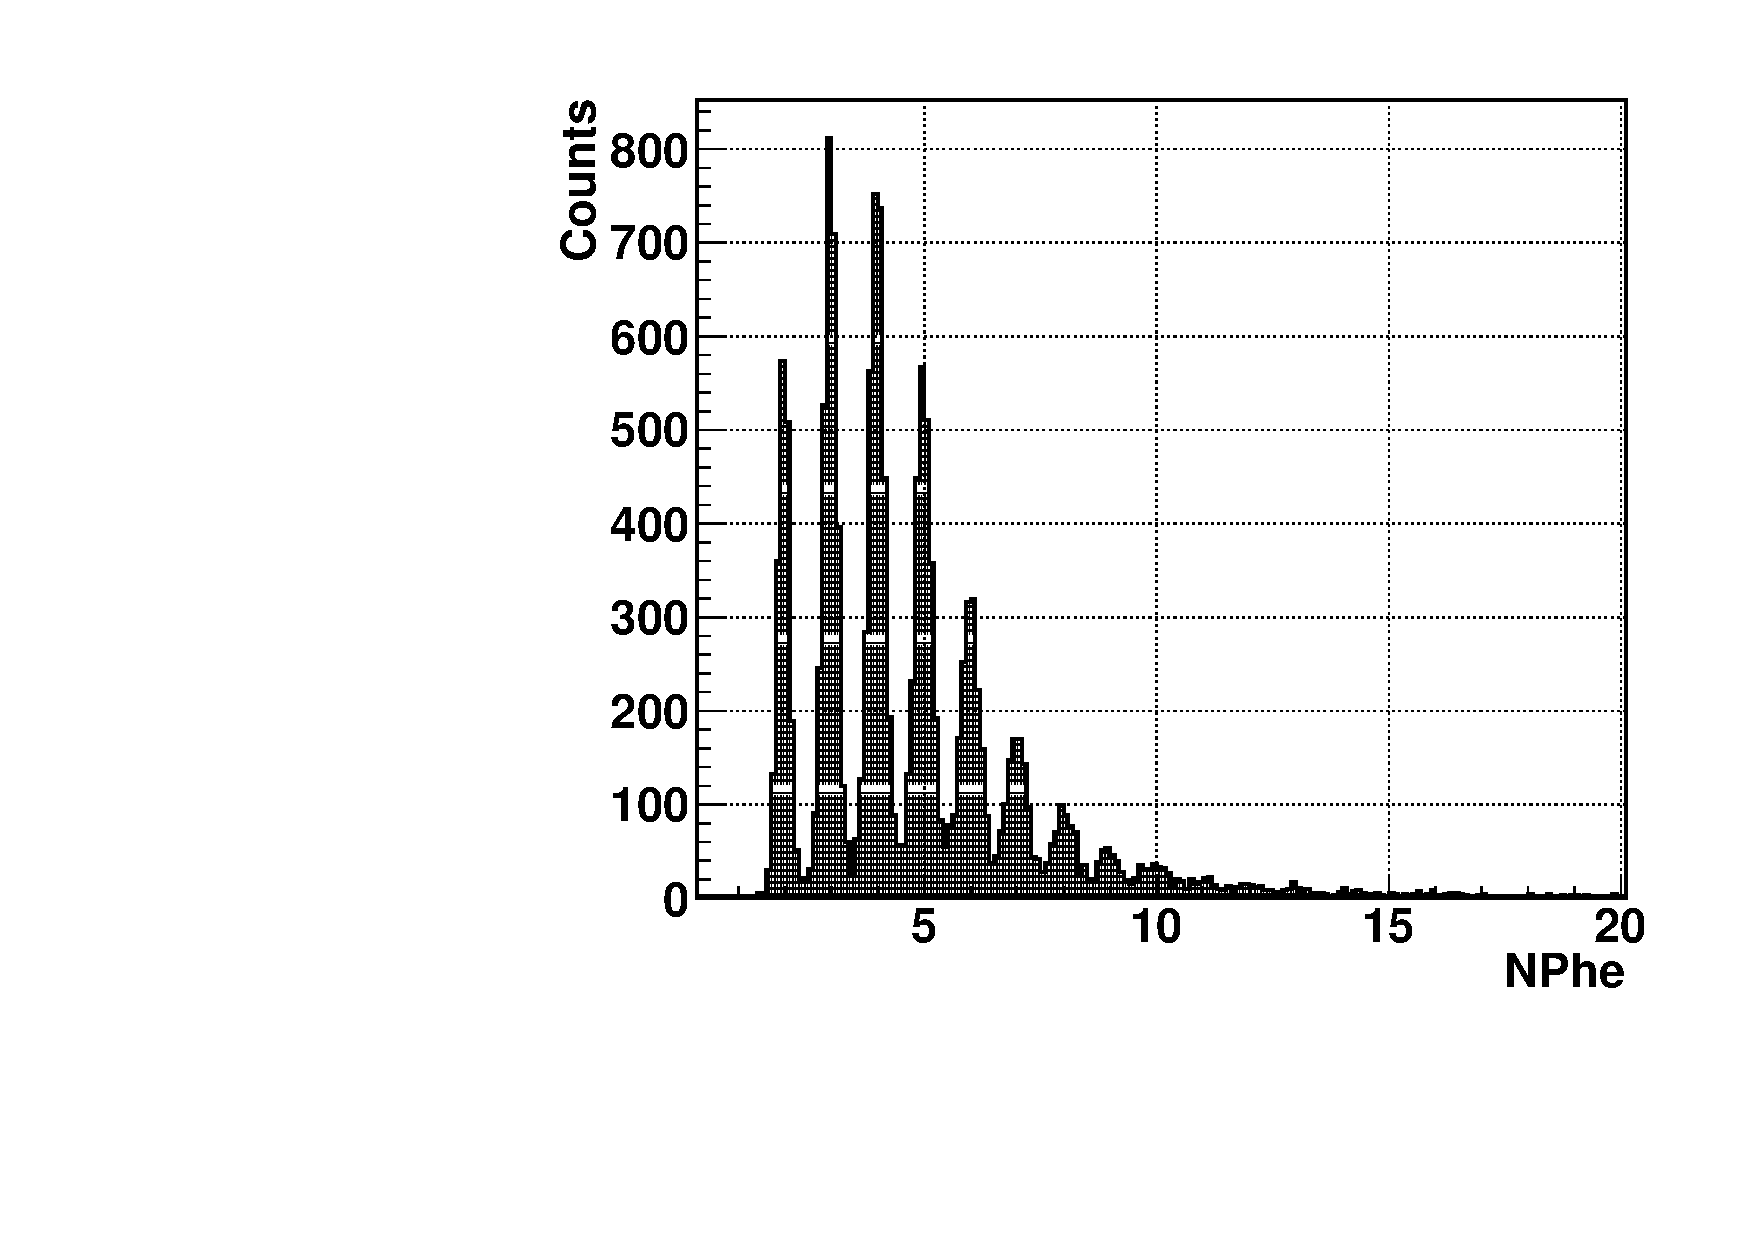
\includegraphics[width=0.48\textwidth]{Figures/muEDM/prototype/prototype_positrons.pdf}\label{fig:ChargeSpectrumAND}}\hfill
            \subfloat[Timing distribution of a single fiber with a double Gaussian fit (solid line).]{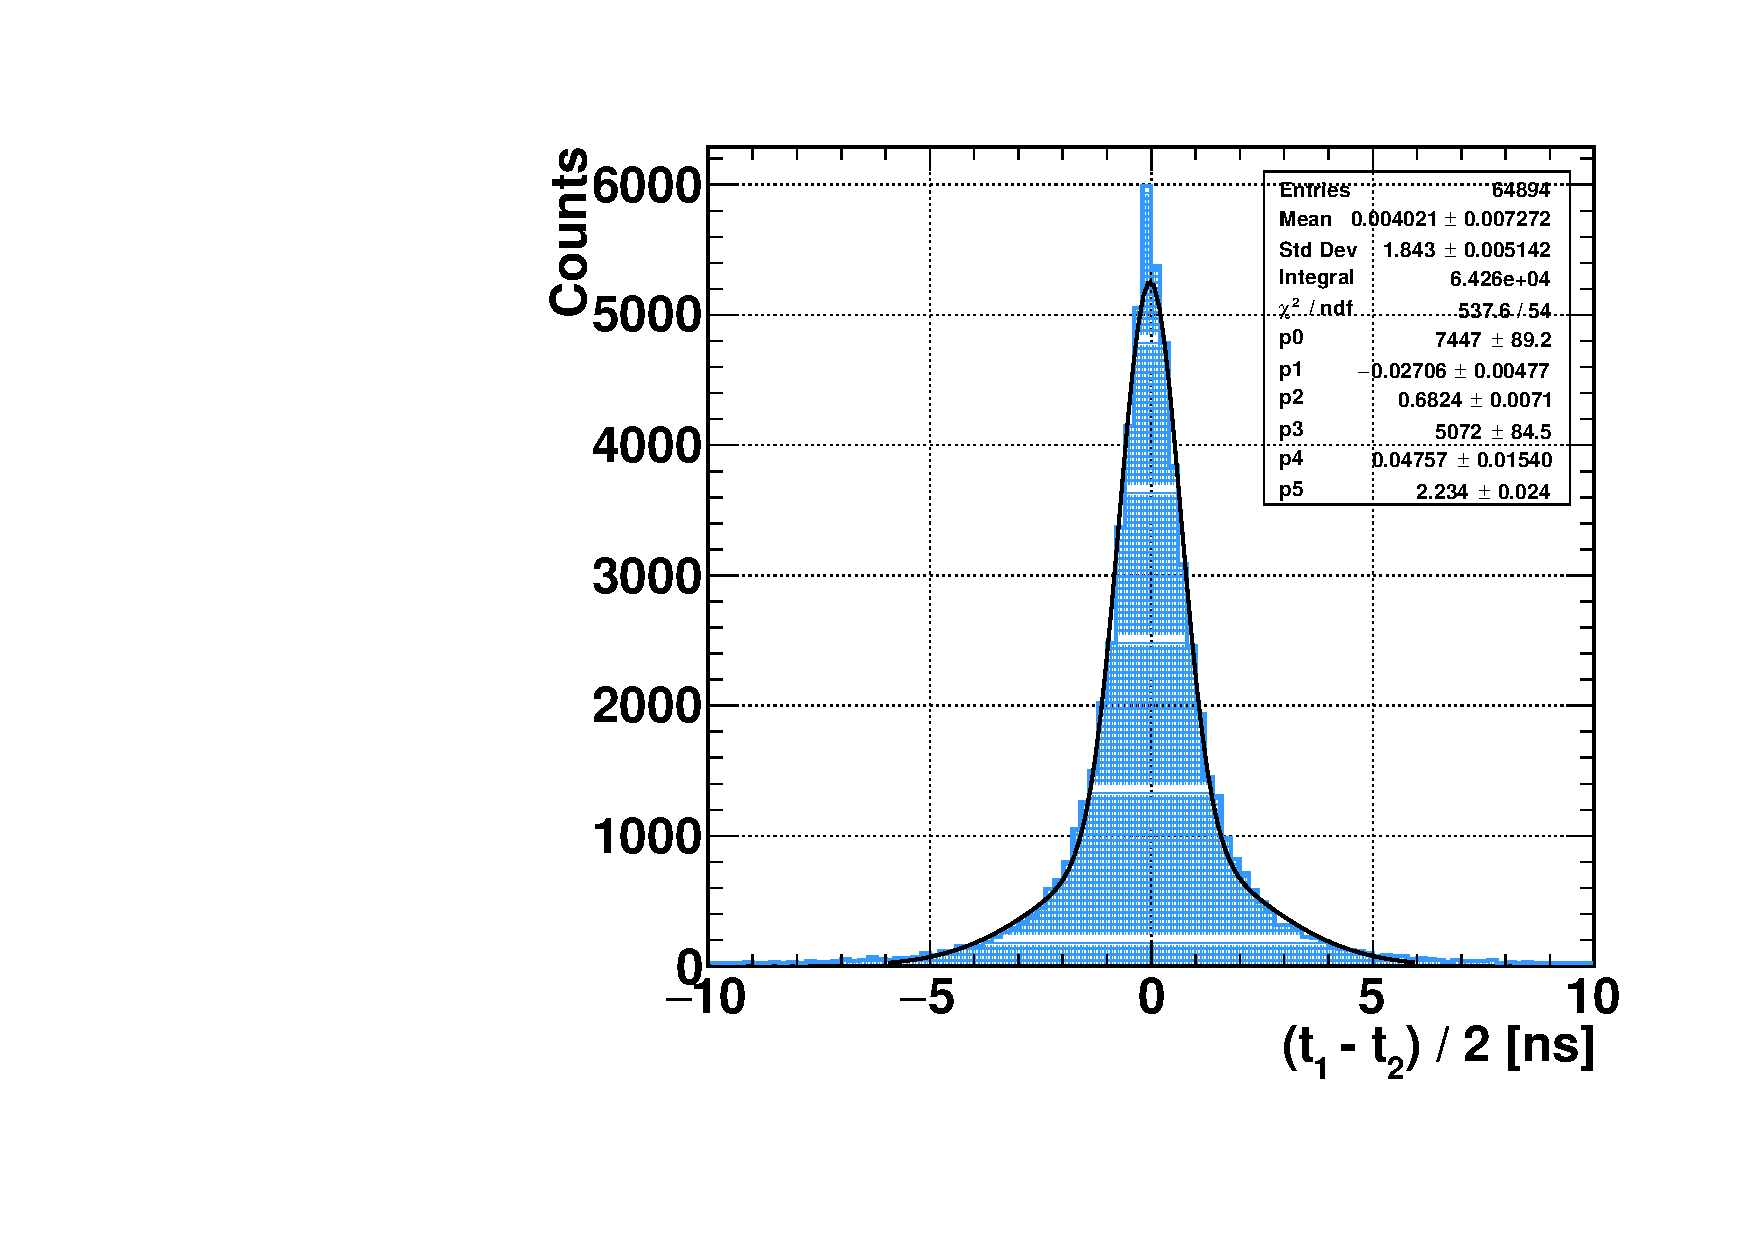
\includegraphics[width=0.48\textwidth]{Figures/muEDM/prototype/prototype_timing.pdf}\label{fig:TimingSingleFibre}}
            \caption[SciFi prototype: light spectrum and time resolution]{Light spectrum and timing resolution of the SciFi prototype}
            \label{fig:enter-label}
        \end{figure}
        
        \begin{table}
        	\begin{center}
        		\begin{tabular}{l | c | c | c | c } 
        		& Single layer & Double layer& Triple layer & Array  \\ \hline\hline
        			   $\varepsilon_{AND}$ [\%] (1.5 phe)  & $34\pm1$ & $52\pm1$ & $67\pm1$ & $88.0\pm0.3$ \\
        			  $\varepsilon_{OR}$ \hspace{0.13cm} [\%] (1.5 phe)    & $79\pm1$ & $93\pm1$ & $97\pm1$ & $97.5\pm0.2$ \\
        			   $\varepsilon_{AND}$ [\%] (0.5 phe) & $72\pm1$ & $89\pm1$ & $95\pm2$ & $95.8\pm0.2$ \\
        			   $\varepsilon_{OR}$ \hspace{0.13cm} [\%] (0.5 phe)   & $96\pm1$  & $99\pm1$ & $98\pm1$ & $98.3\pm0.2$ 
        		\end{tabular}
        	\end{center}	
        		\caption[Detection efficiencies for m.i.p.]{MIP detection efficiencies $\varepsilon_{\rm AND}$ and $\varepsilon_{\rm OR}$ when triggering at the indicated threshold (0.5 or 1.5 phe) on the respective SiPMs in the AND and OR logic. The errors are statistical.}
        		\label{tab:DetectionEff}
        \end{table}

        \noindent
        When a particle hits more than just one fiber, the mean times of the individual fibers can be combined to obtain more precise timing information. Table~\ref{tab:TimingResRibbon} summarizes the measured timing resolutions for different combinations of fibers, which correspond to potentially different thick ribbons, and thresholds. The quoted sigma was obtained with a single Gaussian fit. A better resolution can be quoted using a double Gaussian fit but is beyond the scope of this report. As shown by the measurements, with a ribbon made of three layers of fibers, a timing resolution of \SI{500}{ps} can be achieved with a detection efficiency $\geq90\%$.\\
        
        \begin{table}
        	\centering
        		\begin{tabular}{l | c | c | c }
          			  & Single & Double & Triple \\ \hline\hline
        			  $\sigma_{t}$ [ps] \hspace{0.32cm} (0.5~NPhe) & $1160\pm50$ & $830\pm3$ & $681\pm4$ \\
        			 $\sigma_{t}$ [ps] \hspace{0.32cm} (1.5~NPhe) & $803\pm5$& $600\pm5$ & $504\pm6$  \\
        		\end{tabular}
             \caption[]{Timing resolutions measured by the Large Prototype when triggering at the indicated threshold on the respective SiPMs in the AND logic. The numbers are extracted from single Gaussian fits to the timing spectra. The errors are statistical. }
        	\label{tab:TimingResRibbon}
        \end{table}

        \noindent
        Finally, Fig.~\ref{fig:SciFi_position} shows the tracking capability of the detector with real data. Positrons are impinging at different angles meaning the fired fibers reproduce the particle path. 
        To push the detector performance in this direction, each fiber was coated with a layer of \SI{100}{nm} aluminum before assembling the prototype, reducing optical crosstalk between fibers from around $30\%$ with naked fibers to $\leq1\%$ with coated aluminum fibers.
        
        \begin{figure}
        	\centering
         \begin{minipage}{.3\textwidth}
          \centering	
        		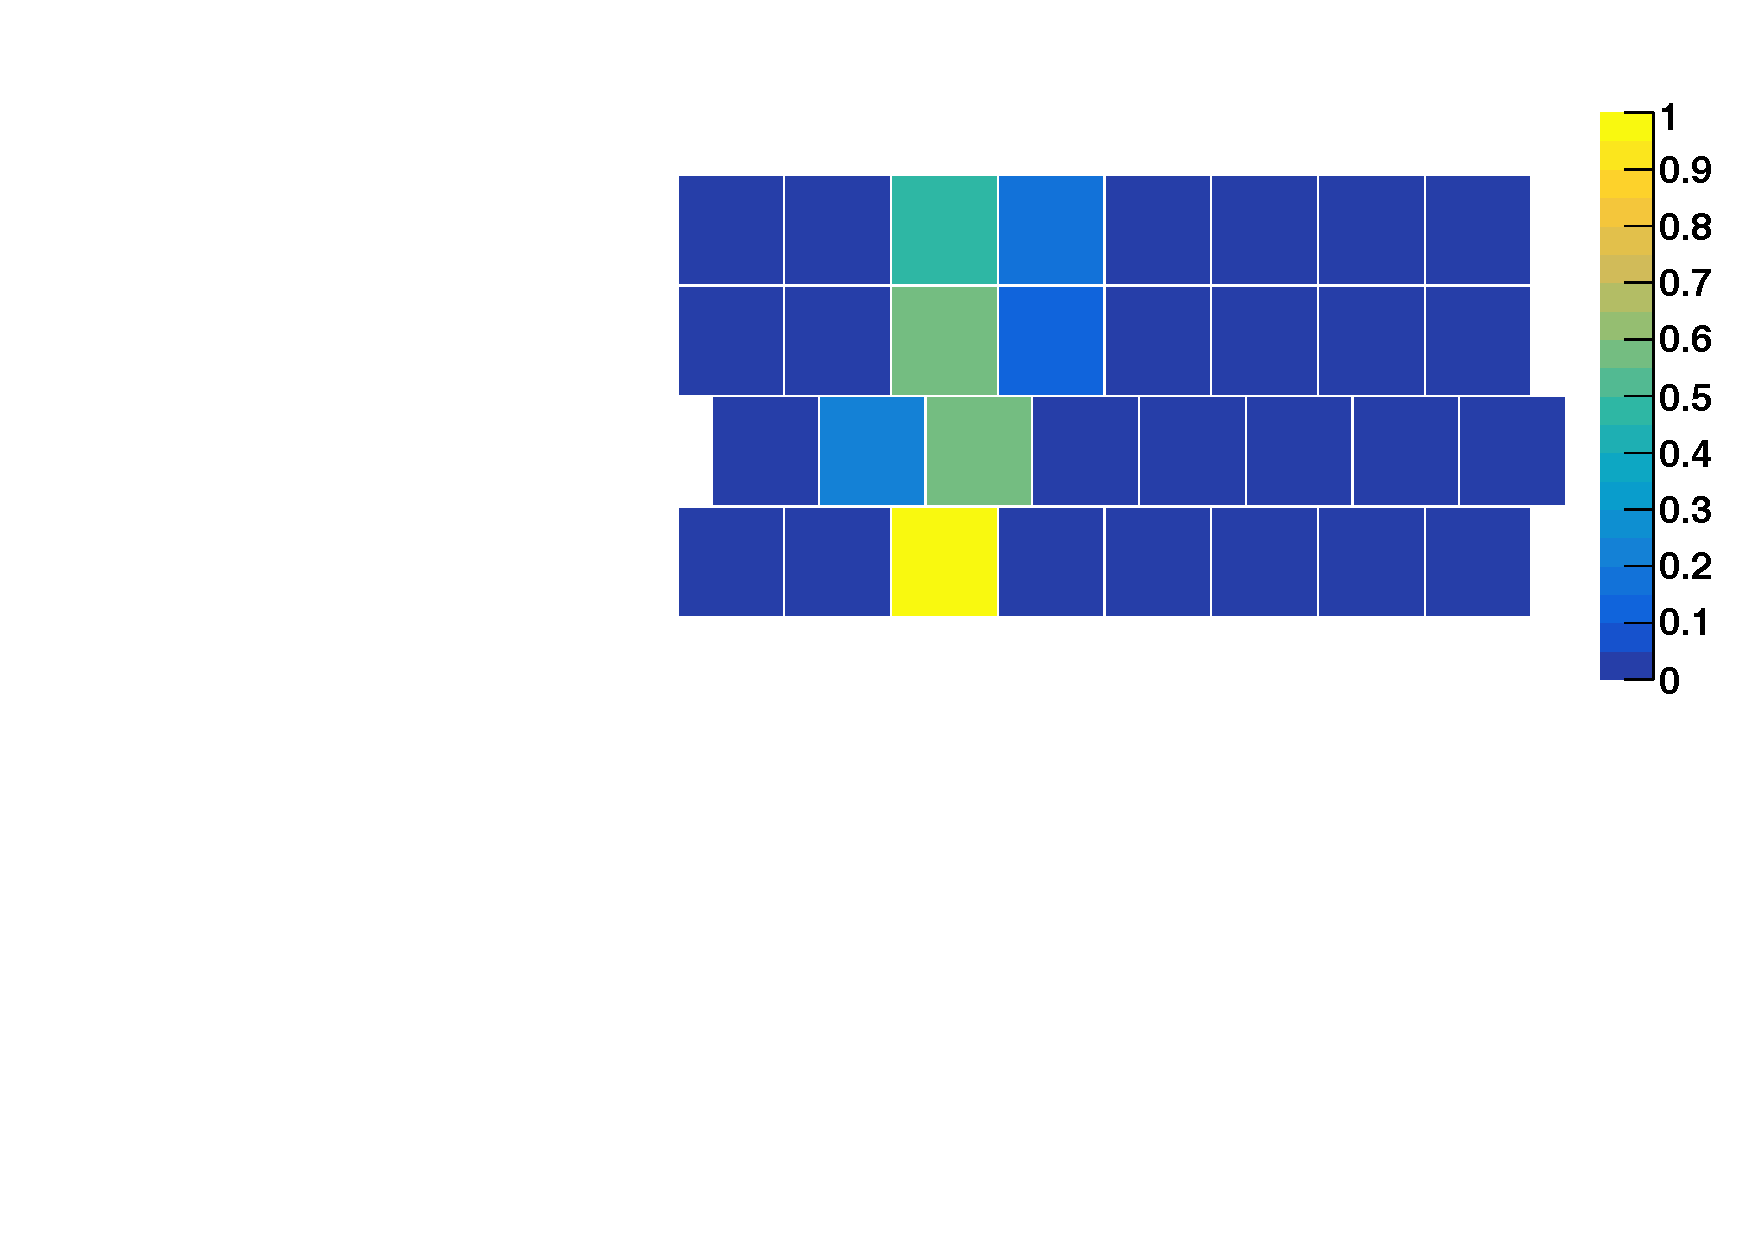
\includegraphics[width=4cm]{Figures/muEDM/prototype/SquaredFiberIlluminationOffset2275.pdf}
        		\label{Ffig:angletracks:0deg}
         \end{minipage}%	
         \begin{minipage}{.3\textwidth}
          \centering		
        		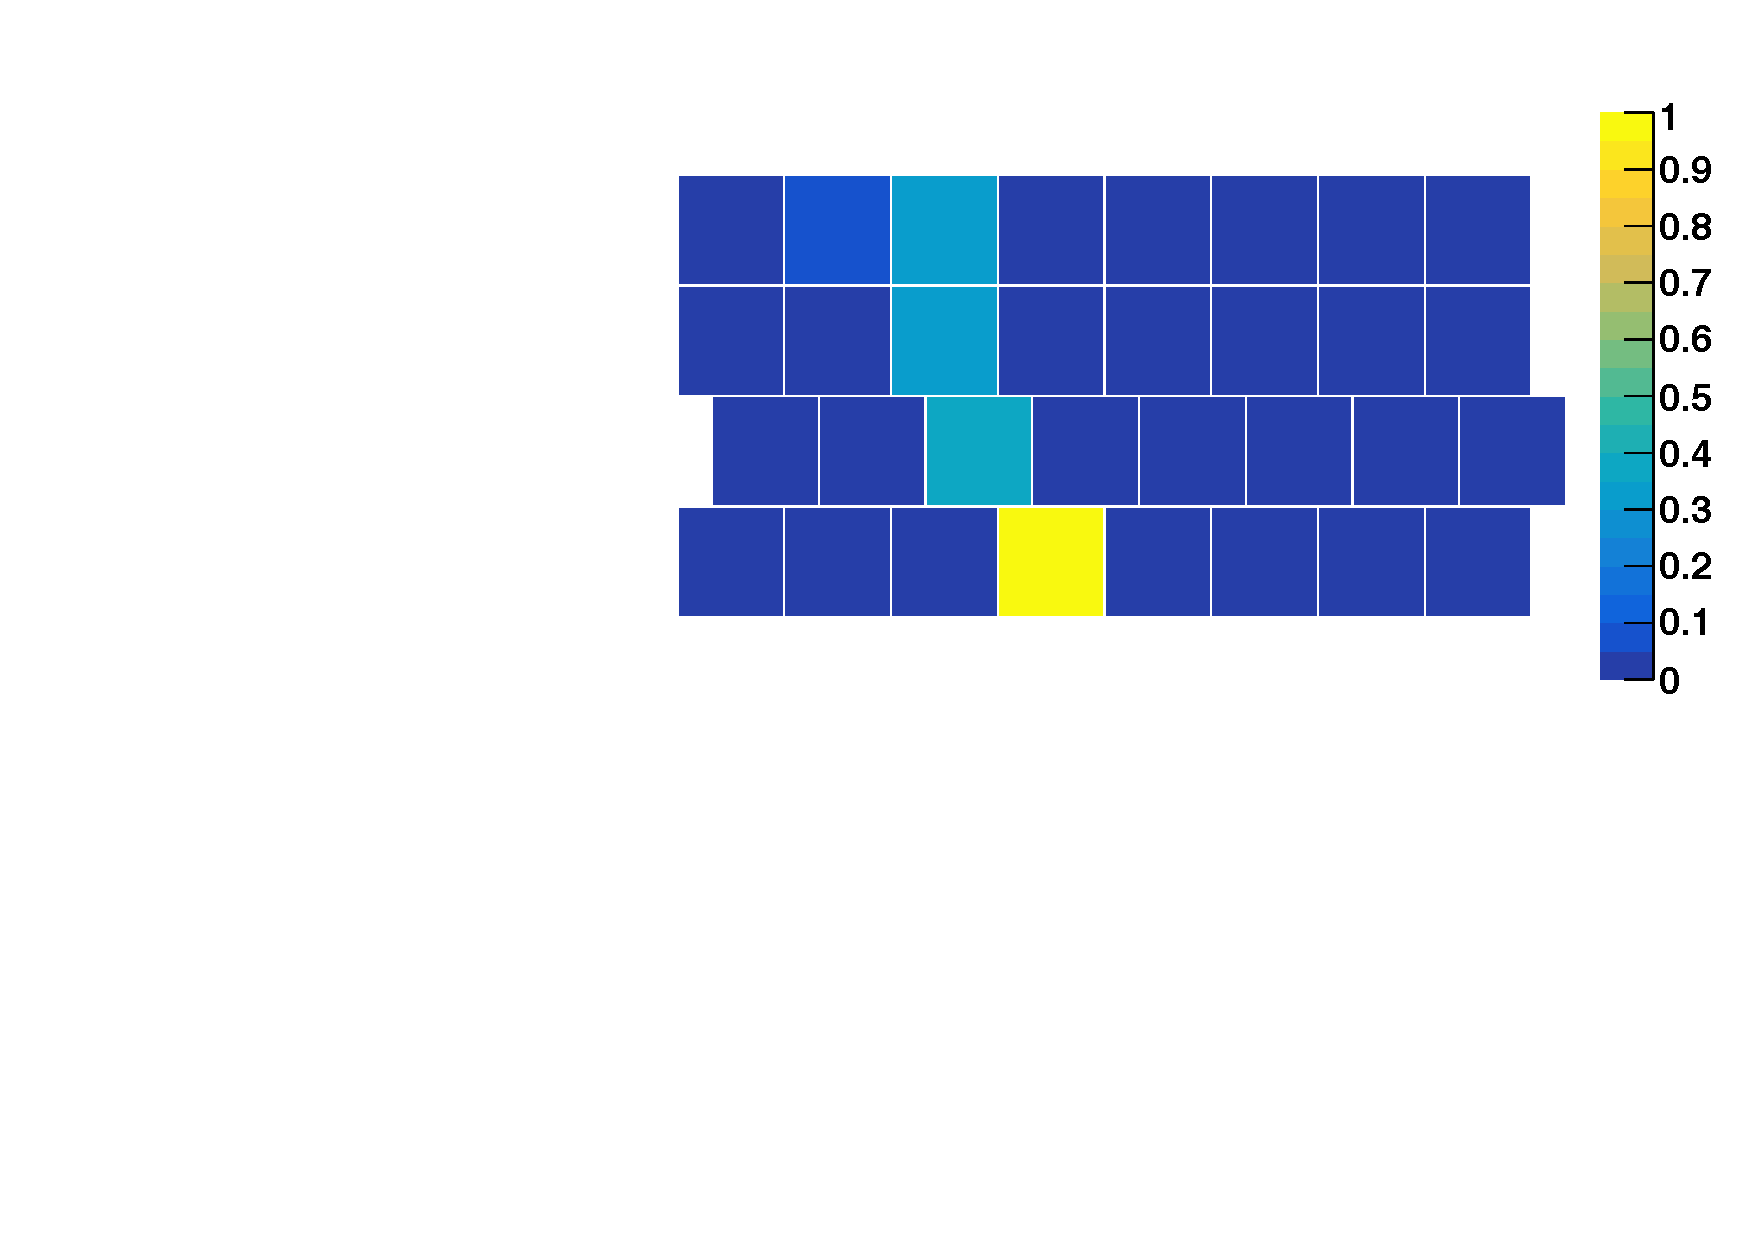
\includegraphics[width=4cm]{Figures/muEDM/prototype/SquaredFiberIlluminationOffset2272.pdf}
        		\label{fig:angletracks:22deg}
        \end{minipage}%	
        \begin{minipage}{.3\textwidth}
          \centering
        		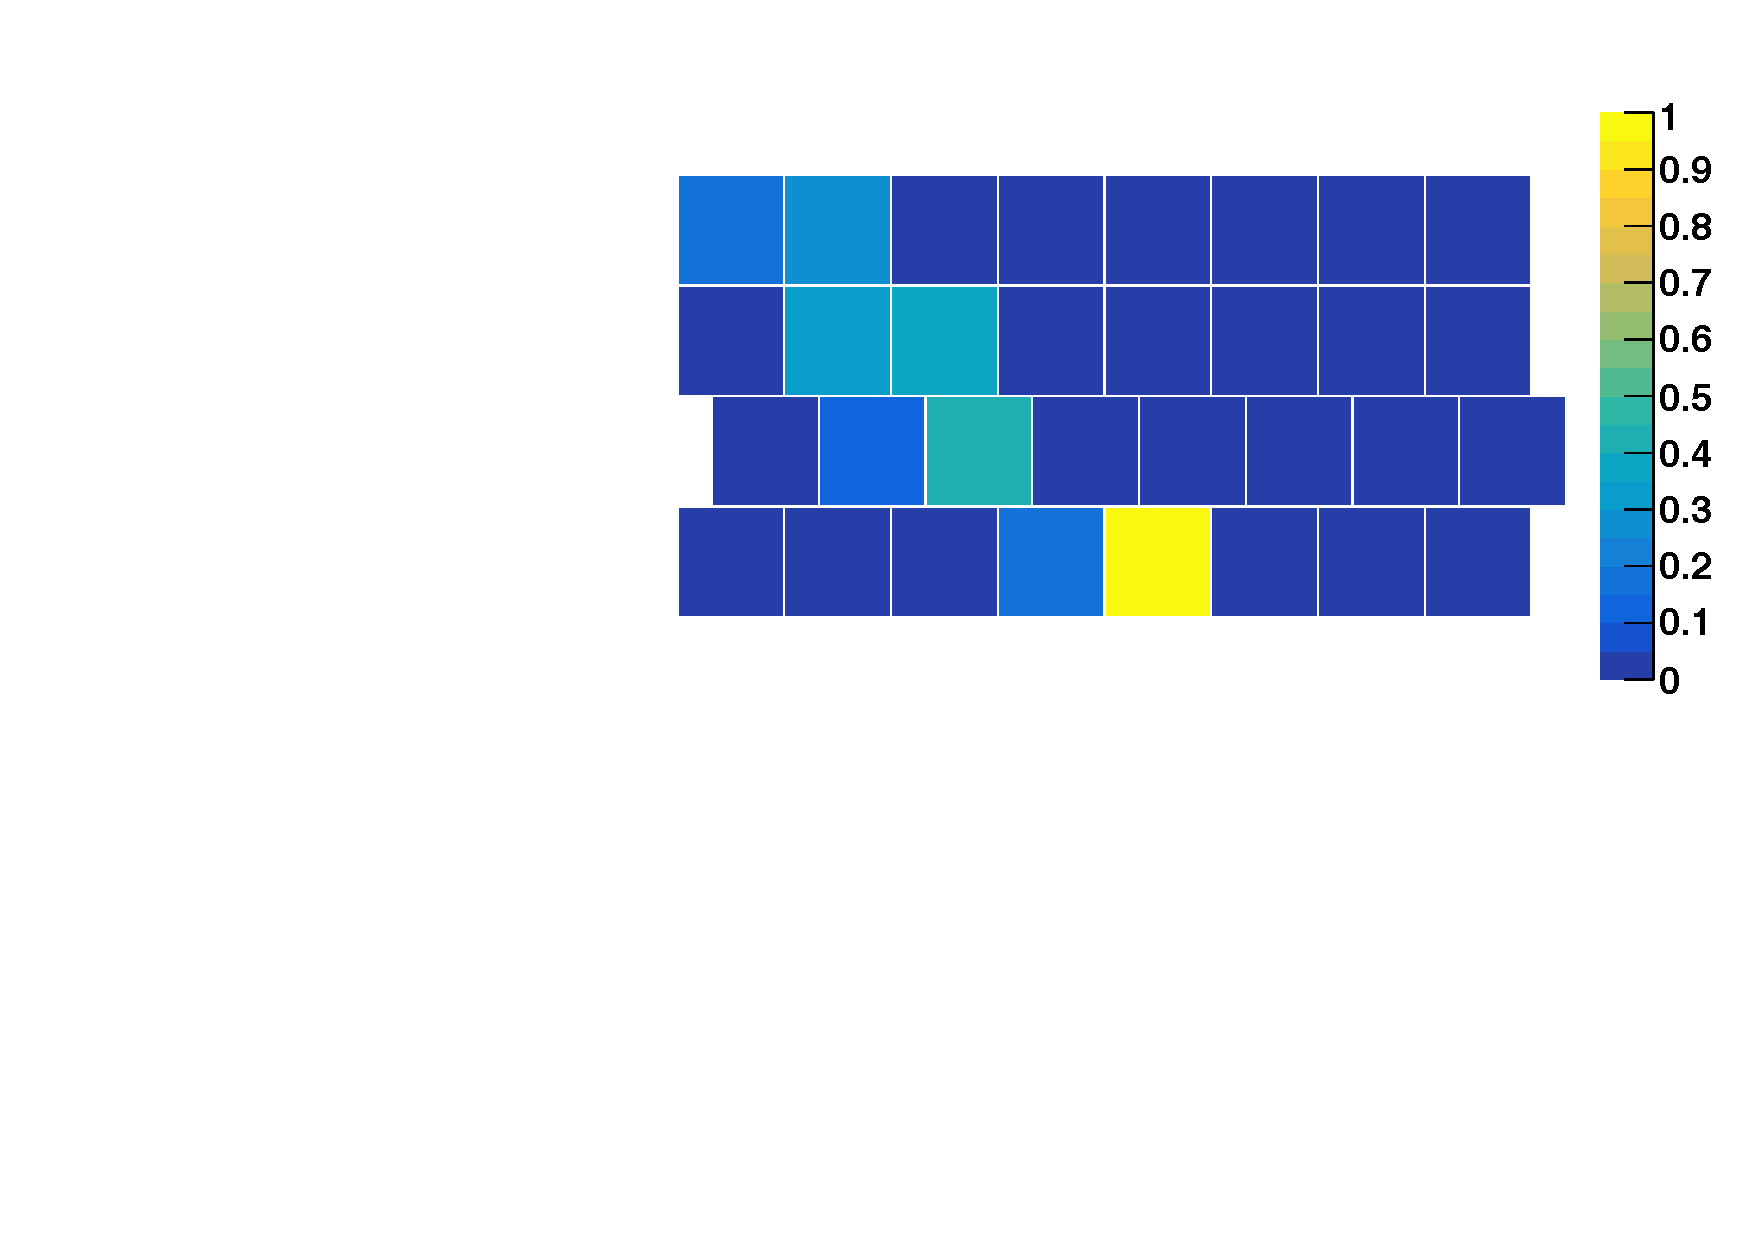
\includegraphics[width=4cm]{Figures/muEDM/prototype/SquaredFiberIlluminationOffset2274.pdf}
        		\label{fig:angletracks:60deg}
        \end{minipage}%	
        \caption[]{Particle tracks observed in the Large Prototype as a function of the inclination angle~$\phi$. From left to right, the impinging angle is $\phi = 0^{\circ}$, $\phi = 22^{\circ}$, and $\phi = 60^{\circ}$. The color scale indicates the number of events involving the corresponding fiber relative to the number of triggered events.}
        \label{fig:SciFi_position}
        \end{figure}
        
    \status{done}
    \subsection{Geant4 simulation and performance}
    \label{sec:muEDM:fiber:g4}
        For current simulations, fiber implementation is based on double-clad BCF20 Saint-Gobain scintillating fiber parameters.
        The sketches of the fiber section and the ribbon are shown in Fig.~\ref{fig:sipmarray:fibercombination}.
        Currently, we are performing simulations that include the interaction between radiation and matter using \textsc{GEANT4} physics processes. 
        Complete photosensor readout and electronics will be implemented once all details of the detector are finalized. 
        At this point, we implemented an ideal readout scenario in which all photons that reach the ends of the fibers are detected and the exact position and timing of each photon are recorded. 
        The idea is to add PDE and smearing offline, simulating different resolutions and efficiencies.
        Additionally, we implemented both a readout scheme 1:1, mimicking a single fiber readout, and a SiPM array system.\\

        \noindent
        As we saw in Sec.~\ref{sec:SciFi_prototype}, we are considering merging multiple fibers into a single photosensor to reduce the number of channels required for the Data Acquisition System (DAQ) of the experiment. 
        However, the performance of the resulting system may be compromised by the balance between the desired resolution and the number of available DAQ channels, as well as by the pixelation of the SiPMs. 
        Despite this, the initial results of tests with a prototype ribbon using a fiber merging readout scheme under realistic conditions (including photosensor response, front-end electronics, and noise) show promising potential to meet muon EDM requirements.

        \paragraph{Fibers and read-out} Aside from the specific geometry, the cardinal point is how to describe the fibers and their readout. 
        The fiber itself is simulated as a three-layer volume: a scintillating core and two claddings of PMMA.
        The optical property of the surface between the different layers is specified with a G4OpticalSurface\footnote{The documentation can be found here: \href{https://apc.u-paris.fr/~franco/g4doxy/html/classG4OpticalSurface.html}{https://apc.u-paris.fr/~franco/g4doxy/html/classG4OpticalSurface.html}}.
        The readout is a somewhat simplified simulation of a SiPM (the same one used also for the different scintillators discussed in the previous chapter):
        \begin{outline}
            \1 Optical grease: to simulate the optical coupling of the SiPM to the fibers/scintillators
            \1 SiPM window: SiPMs have a Silicon resin window covering the active region
            \1 SiPM: The bulk of the SiPM is simulated as a simple block of silicon
        \end{outline}
        The idea of this readout is not to simulate the actual physical processes leading to an electric signal, but just to record the position and time of optical photons entering the system.

        \subsubsection{Signle ribbon}
        The first step is to study the characteristics and performance of a single ribbon. Having two impinging particles at the same time at a given distance, we can estimate the spatial resolution of this system.  Fig.~\ref{fig:geant4_position_resolution} shows an event with two particles separated by \SI{2}{mm}. Looking at the position of the generated photons, we can clearly distinguish the two hits, and the resolution is of the order of \SI{0.1}{mm}.
        In Fig.~\ref{fig:geant4_time}, the arrival time of the scintillating photons at the photosensor, generated by two consecutive particles, is shown. 
        The position of the impinging particles is the same, but a different $\Delta t$ was set between them. 
        Although the time resolution for a single particle is given by the rising edge of the distribution, much sharper than required $\sim \SI{1}{ns}$, the distribution itself is quite broad. 
        This means that a particle that crosses at the same position within $\lesssim$ \SI{3}{ns} will induce a pile-up event. 
        Note that here we neglect the shaping of the waveform, for which a bigger width is expected. 
        Although with a short time difference, the hits might not be recognizable, the resulting distribution would still be quite different from that of a single impinging particle, and this feature could be somewhat mitigated. 
        The probability of having no deflection due to multiple scattering on a full rotation is quite low: the spatial resolution will further mitigate this pile-up effect. 
        
        \begin{figure}
            \centering
            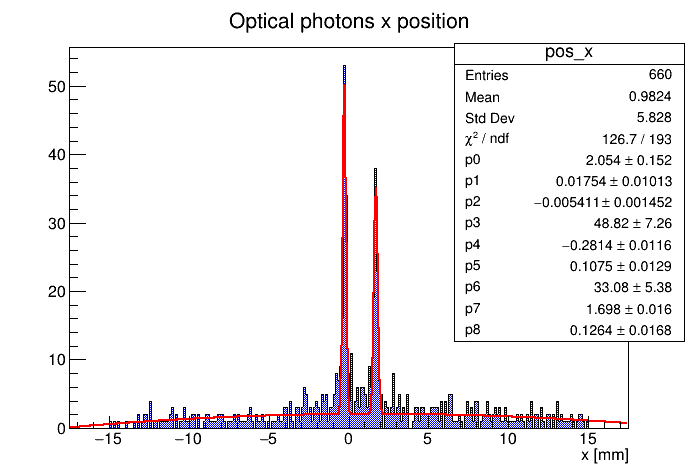
\includegraphics[width=0.5\textwidth]{Figures/muEDM/Tracker/2mm.png}
            \caption[SciFi \gf: spatial resolution]{Two particles impinging \SI{2}{mm} apart on the same ribbon. Using \SI{250}{\micro m} fibers and having no pixelation on the readout, the spatial resolution is $\sigma\approx \SI{100}{\micro m}$ (p5 and p8). This value was obtained with a fit to \textit{plo2+gauss+gauss} and with a bin width of \SI{125}{\micro m} (half a fiber width).}
            \label{fig:geant4_position_resolution}
        \end{figure}
    
        

        \begin{figure}
            \centering
            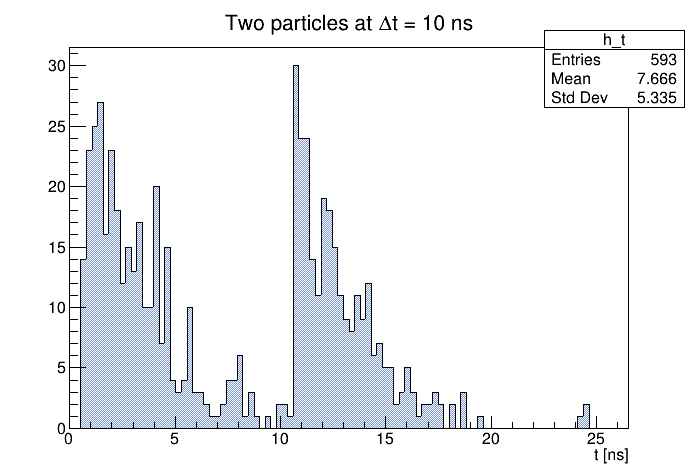
\includegraphics[width=0.32\textwidth]{Figures/muEDM/Tracker/10ns.png}
            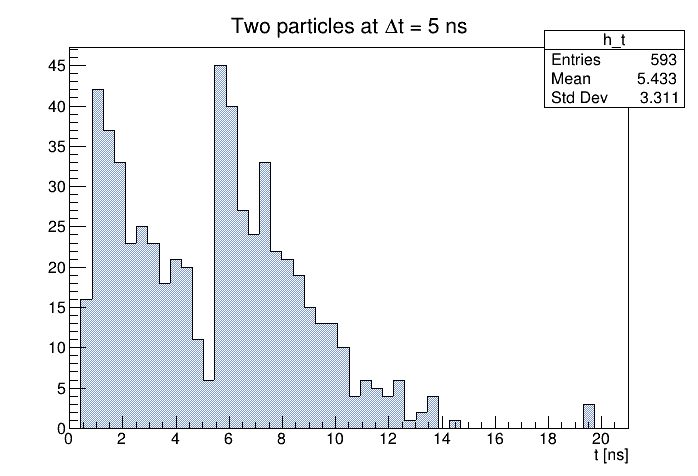
\includegraphics[width=0.32\textwidth]{Figures/muEDM/Tracker/5ns.png}
            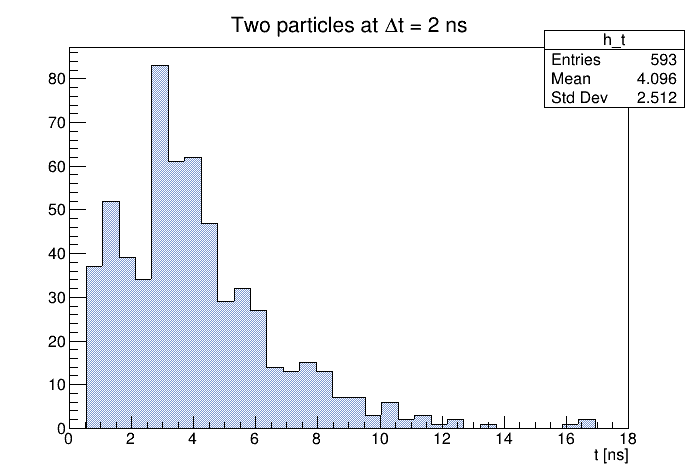
\includegraphics[width=0.32\textwidth]{Figures/muEDM/Tracker/2ns.png}
            \caption[SciFi \gf: time resolution]{In case of a particle impinging on the same position, the timing of the photon can be used to distinguish the two hits. For \SI{20}{cm} fibers, the limit seems to be \SIrange{3}{5}{ns}. This value refers to the time the optical photon interacts with the SiPM. The actual distribution will be larger.}
            \label{fig:geant4_time}
        \end{figure}

        \subsubsection{MuEDM geometry}
        Simulating the full geometry, including both the inner layer of transverse fibers and the outer layer of longitudinal fibers, leads to more complex events. 
        An example is shown in Fig.~\ref{fig:geant4_B}. In this scenario, a single particle can pass through multiple layers, undergoing scattering and losing energy. 
        The spatial information provided by both layers, as shown in Fig.~\ref{fig:geant4_position}, demonstrates that the positions of the hits on the transverse plane are relatively stable, due to the low material budget. On the contrary, the inner layer provides information about the longitudinal movement of the particle.
        The integration of timing information for the transverse fibers results in the plot shown in Fig.~\ref{fig:geant4_time_pos}. This plot includes horizontal lines that represent the separation between different barrels. 
        The relationship between transverse position and time provides additional information, although it can be more difficult to interpret. 
        The resulting plots are shown in Fig.~\ref{fig:geant4_time_pos_transverse}.

        \begin{figure}
            \centering
            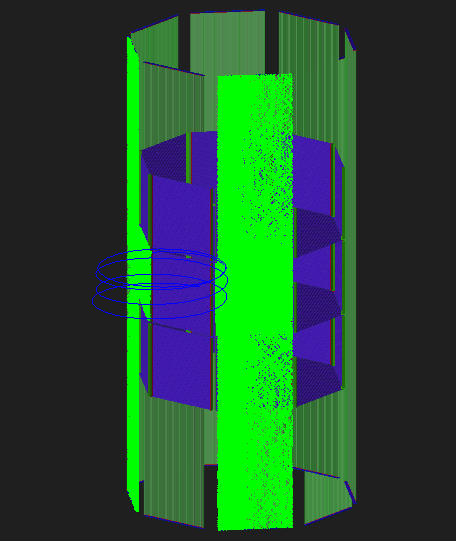
\includegraphics[width=0.5\textwidth]{Figures/muEDM/Tracker/muedm_scifi_B.png}
            \caption[SciFi \gf: muEDM geometry from the proposal]{An example of a \textsc{GEANT4} simulated event. In green the optical photons reflect inside the fiber ribbons; in blue the trajectory of the positron. Keeping the same color scheme, the longitudinal SciFi is green while the transverse one is blue.}
        \label{fig:geant4_B}
        \end{figure}

        \begin{figure}
            \centering
            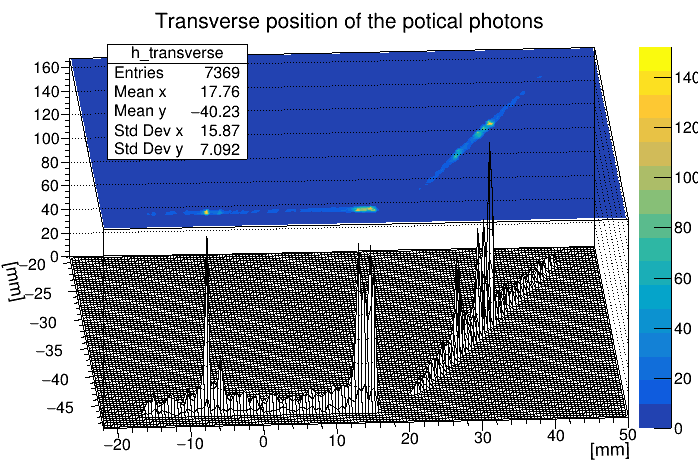
\includegraphics[width=0.49\textwidth]{Figures/muEDM/Tracker/fPosInXfPosInZ.png}
            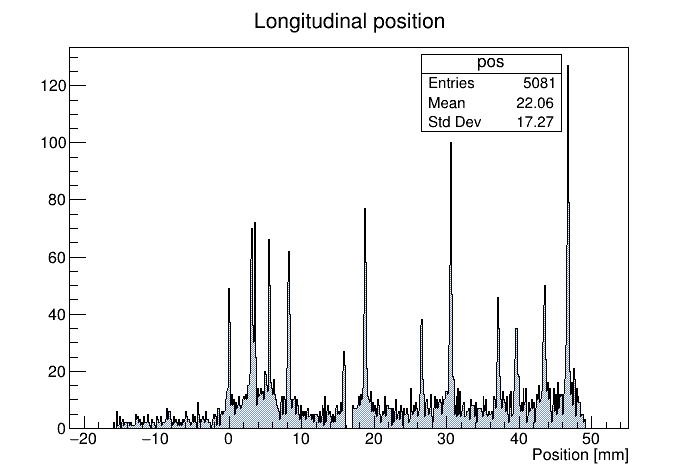
\includegraphics[width=0.49\textwidth]{Figures/muEDM/Tracker/fPosInY.png}
            \caption[muEDM tracker \gf: transverse and longitudinal information]{Looking at the position for the photons arriving at the readout for both SciFi layers.}
        \label{fig:geant4_position}
        \end{figure}
    
        \begin{figure}
            \centering
            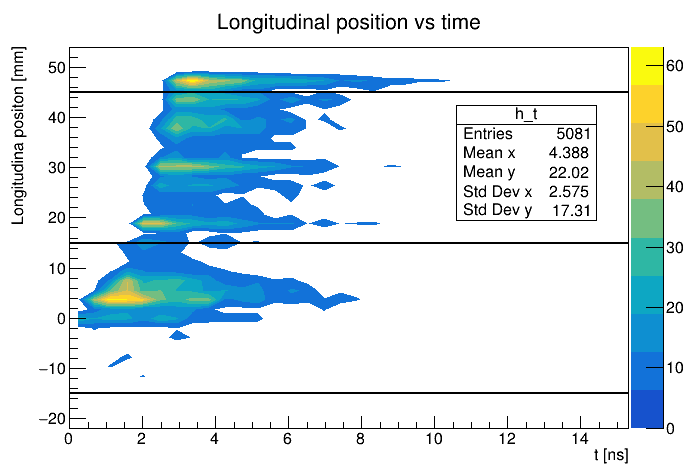
\includegraphics[width=0.8\textwidth]{Figures/muEDM/Tracker/fPosInYfTimeIn.png}
            \caption[muEDM tracker \gf: time and logitudinal position]{Looking at the relationship between time and longitudinal position for the inner layer makes it possible to see if the particle is spiraling up or down.}
        \label{fig:geant4_time_pos}
        \end{figure}

        \begin{figure}
            \centering
            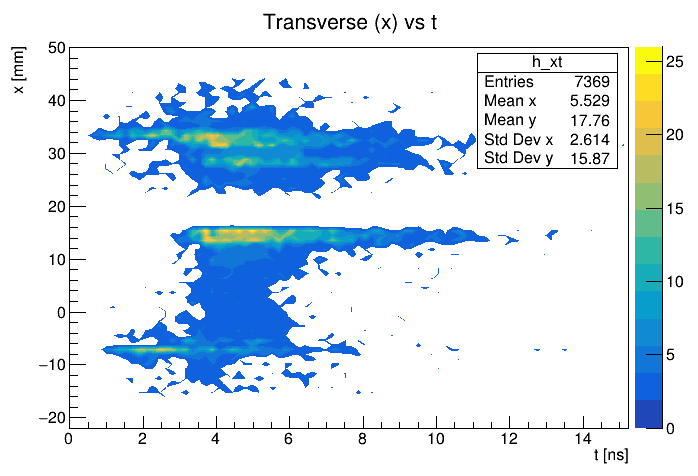
\includegraphics[width=0.49\textwidth]{Figures/muEDM/Tracker/fPosInXfTimeIn.png}
            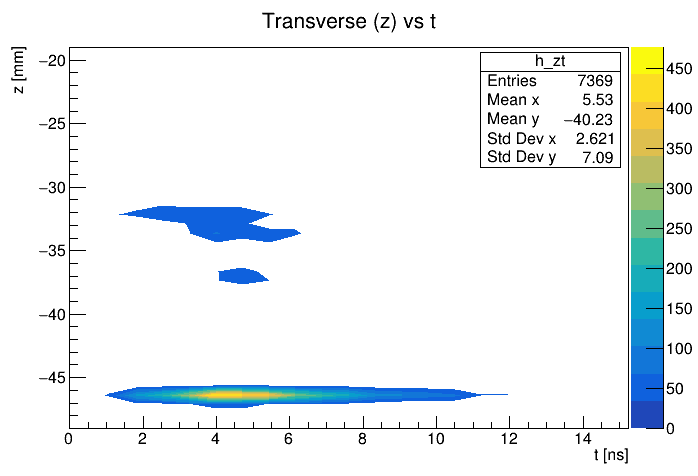
\includegraphics[width=0.49\textwidth]{Figures/muEDM/Tracker/fPosInZfTimeIn.png}
            \caption[muEDM tracker \gf: combined information]{The information from the joint use of transverse position and time, given by the outer layer, is more complex but essential (and a unique feature of this detector) in understanding the particle trajectory.}
        \label{fig:geant4_time_pos_transverse}
        \end{figure}

    \status{done}
    \subsection{Conclusions on the 2022 proposal}
        The tracker technology and geometry illustrated are a preliminary design, but already meet the requirements of positron tracking, i.e. millimeter and nanosecond resolutions. 
        The interplay of a transverse SciFi detector and a silicon-based longitudinal detector seems to be a desirable choice. 
        Working under this assumption, we envision the possibility of removing the longitudinal outer SciFi, which would be redundant, further reducing multiple scattering. 
        On a practical level, this system requires finding a way of reading the transverse fibers from the central region of the experiment.
        This is non-trivial and possible improvements on this design were studied, the most promising being the Cylindrical Helical Tracker (CHeT), discussed in the next section.
        
\status{done}
\section{CHeT}
    The first step in further developing and prototyping the geometry chosen in the previous paragraph is to understand the requirements for this sub-detector and how the prospected resolutions compare to these.
    This scintillating fiber tracker will be used for position tracking and in particular is going to be complemented by silicon strips. The crucial information this system needs to provide is the longitudinal position of the particle with a good resolution: $\delta \ell \lesssim \SI{1}{mm}$.

    \status{done}
    \subsection{Resoutions of crossed fibers ribbons}
        Let's consider a ribbon  $\SI{3}{cm}\times\SI{15}{cm}$ of squared fibers \SI{250}{\micro m} running vertically. Assuming a `perfect' readout, the resolution across the ribbon is given simply by the fibers' width while the resolution along the ribbon is extracted by reading the fibers on both sides. This second resolution is often quite worse than the previous. For practical purposes we will here assume $\delta_x = \SI{1}{mm};\ \delta_y = \SI{10}{mm}$.
        Rotating the ribbon by an angle $\theta$ changes the projection of the resolutions on the $\hat{x},\ \hat{y}$ axes and for this reason crossing two ribbons can improve the resolutions on the position of a crossing particle.
        When reading the ribbon on both sides the resolutions, as a function of $\theta$, are given by the smaller between the projection of the two intrinsic resolutions.  
        \begin{equation}
            \begin{cases}
            \dd x = min(\delta x \sec \theta;\ \delta y \csc \theta)\\
            \dd y = min(\delta x \csc \theta;\ \delta y \sec \theta)
            \end{cases}
        \end{equation}
        The relation between resolutions and the tilt angle is shown in fig. \ref{fig:CyFi:examples:b}.  

    \status{done}
    \subsection{Angle choices for the layers}
    \label{sec:muEDM:CHeT:crossed}
        When considering two layers the angles must be chosen to improve the overall resolution, which in practice means minimizing the uncertainty only on one axes per ribbon.
        Let's consider the different layouts in \ref{fig:CyFi:examples:a} and how they translate to resolutions in \ref{fig:CyFi:examples:b}.
        Clearly having the two ribbons at \SI{90}{\deg} along the axes is the best option but if we want to avoid having the readout on the plane of the muon orbit we need to consider less steep angles for the single ribbons.
        Options C and D are the possible solutions and, looking at the resolutions, D is actually the configuration minimizing the resolutions on both axes. 

    \status{done}
    \subsection{Cylindrical geometry}
    \label{sec:muEDM:CHeT}
        At this point is important to notice an additional constraint, given by the cylindrical geometry.
        If, instead of having planar ribbons, the fibers are woven into two concentric cylinders one needs to avoid having multiple crossings.
        If two fibers cross multiple times, when both are scintillating the position of the impinging particle is ill-defined. There is a `real' crossing point but also additional \textit{ghosts} hits.
        If we consider a two-layer system the requirement of having only one crossing point (i.d. no ghosts) translates to having a difference in the number of turns $\lesssim1$. 
        In a cylindrical geometry the relation between the angle of the fibers and the number of turns completed, shown in Fig.~\ref{fig:CyFi:TurnsVsAngles}, is determined by the dimensions of the cylinder itself.
        At this point, we can plot the resolutions as a function of the angle of one of the layers keeping the angle of the second layer such as $\Delta T=1$. 
        The results are in Fig.~\ref{fig:CyFi:projected_dxdy} while Fig.~\ref{fig:CyFi:angle} shows the difference in the angle of the two layers.
        We will consider two concentric cylinders, the outer layer being the one with a shallower angle: this is intended to reduce the effect of multiple scattering on the longitudinal position. 
        Given its details, this detector has been named \textbf{C}ylindrical \textbf{He}lical \textbf{T}racker (CHeT).
        
        \begin{figure}
            \subfloat[Some possible orientation for two ribbons.]{
            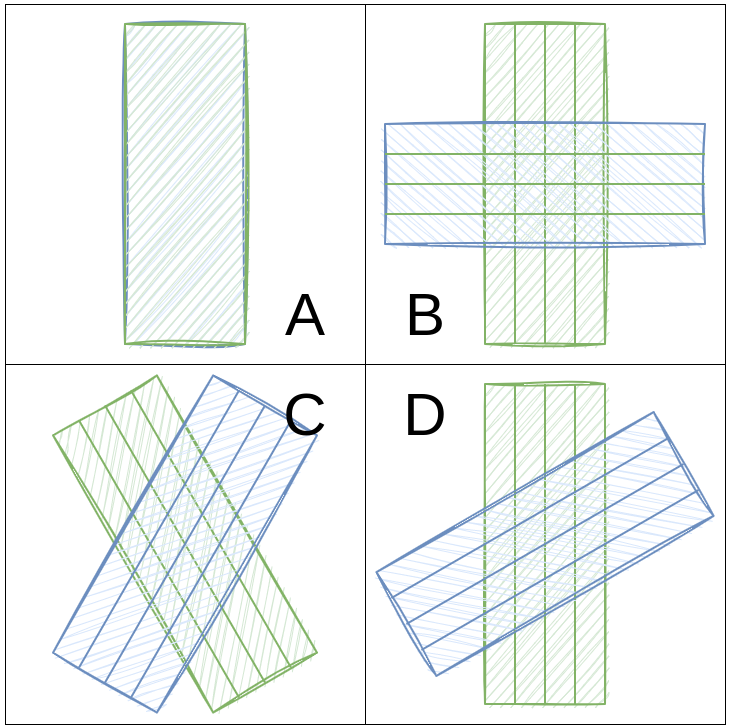
\includegraphics[width=0.41\textwidth, keepaspectratio]{Figures/muEDM/CyFi/CrossingFibres_config.png}
            \label{fig:CyFi:examples:a}}
            \subfloat[Projected uncertainties as a function of the outer layer's angle]{
            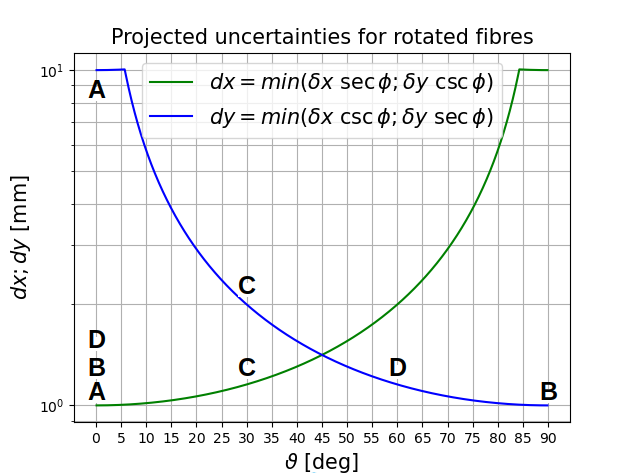
\includegraphics[width=0.57\textwidth, keepaspectratio]{Figures/muEDM/CyFi/projected_dxdy_examples.png}
            \label{fig:CyFi:examples:b}}
            \caption[CHeT: angle-resolution study]{Relation between the direction of the fibers and the projection along the $\hat{x};\ \hat{y}$ axes of the resolutions. The intrinsic resolutions are here assumed $\delta_x = \SI{1}{mm};\ \delta_y = \SI{10}{mm}$.
            Some specific orientations of two overlapping ribbons are shown in both (a) and (b).}
        \end{figure}
        
        \begin{figure}
            \centering
            \subfloat[Number of turns as function of the angle of the fibers]{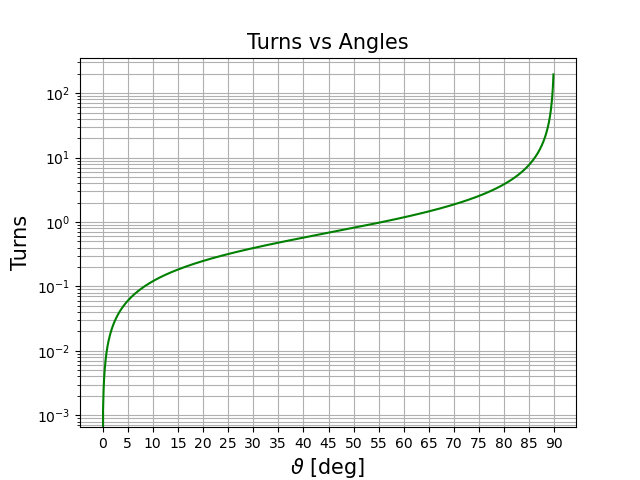
\includegraphics[height = 7.5cm]{Figures/muEDM/CyFi/TurnsVsAngles.png}\label{fig:CyFi:TurnsVsAngles}}\hfill
            \subfloat[A 3D representation of the system.]{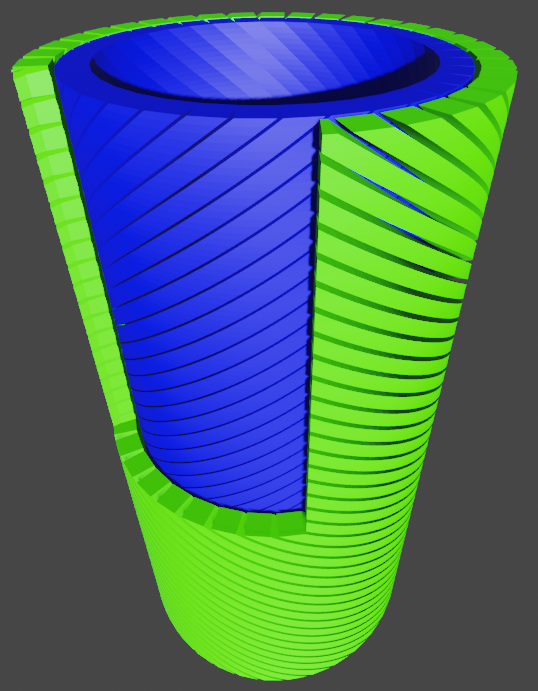
\includegraphics[height = 7.5cm]{Figures/muEDM/CyFi/muedm_CyFi2.png}\label{fig:CyFi:3D}}
            \caption[CHeT: angle and number of turns]{In a planar configuration, the angle at which the fibers run translates directly to the angle at which the ribbon is oriented. In a cylindrical geometry, a fiber running at a given angle will complete a different number of turns depending on the dimensions of the cylinder. in (b) a 3D view with two layers in opposite directions. To make it easier to read the fibers are wider than in reality.}
        \end{figure}
        \begin{figure}[ht]   
            \centering
            \subfloat[Projected uncertainties as a function of the outer layer's angle]{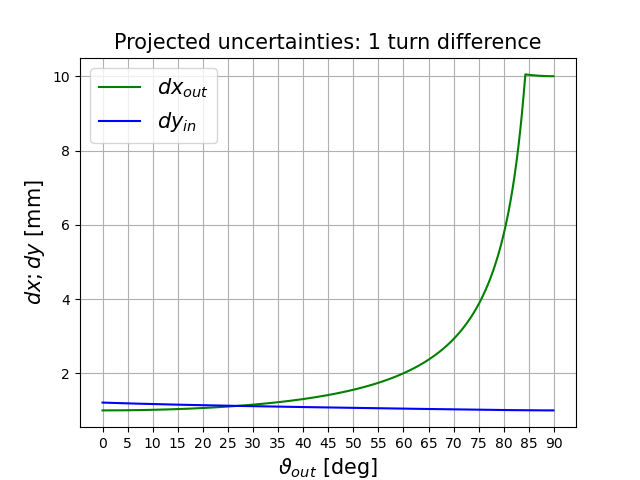
\includegraphics[width=0.49\textwidth, keepaspectratio]{Figures/muEDM/CyFi/projected_dxdy_1Turn.png}\label{fig:CyFi:projected_dxdy}}
            \hfill
            \subfloat[Angle of the inner layer and difference in angle as a function of the angle of the outer layer]{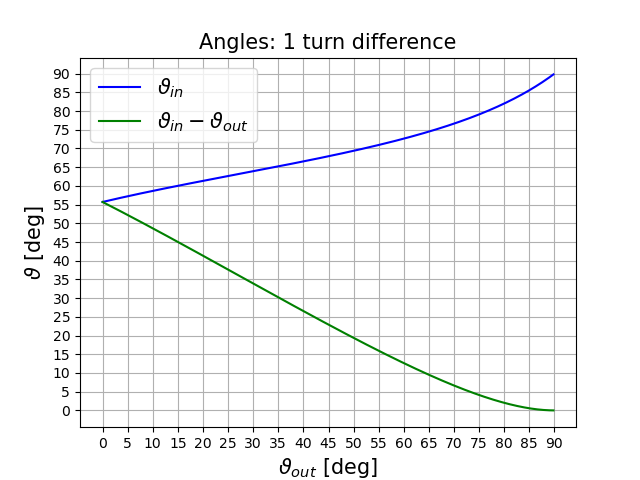
\includegraphics[width=0.49\textwidth, keepaspectratio]{Figures/muEDM/CyFi/Angles_1Turn.png}\label{fig:CyFi:angle}}
            \caption[CHeT: resolution and angles for $\Delta T=1$]{The results when considering two layers in a cylindrical geometry keeping the requirement $\Delta T=1$: \ref{fig:CyFi:projected_dxdy} shows the projected uncertainties; \ref{fig:CyFi:angle} shows the angle of the inner layer.}
            \label{fig:CyFi}
        \end{figure}
        
        \noindent
        Building the layers with infinite precision on the angle is clearly not feasible for this reason we can use the plots in Fig.~\ref{fig:CyFi:5deg}, where the angles have been rounded to multiples of \SI{5}{\deg}. 
        Additional attention we can have is to consider the length of the scintillating fibers: if the fibers are too long the light collection at the ends is decreased by the absorption. The length of the fibers in both layers is shown as a function of the outer angle in Fig.~\ref{fig:CyFi:5deg:length}.
        Depending on the intrinsic resolutions of the fibers, shallower angles and $\Delta T<1$ could be chosen, simplifying the construction.\\
        
        \noindent
        The concepts here introduced are true for the system envisioned, but the specific values obtained depend on the specific dimensions of the cylinder as well as the intrinsic resolutions of a ribbon of fibers. 
        For the plots shown, we considered a cylinder of $r=\SI{3.1}{cm}$ and $h=\SI{20}{cm}$, reasonable sizes for the task at hand, and the intrinsic resolutions are here assumed $\delta_x = \SI{1}{mm};\ \delta_y = \SI{10}{mm}$.
        
        \begin{figure}[ht]   
            \centering
            \subfloat[Angle of the inner layer and difference in angle as a function of the angle of the outer layer]{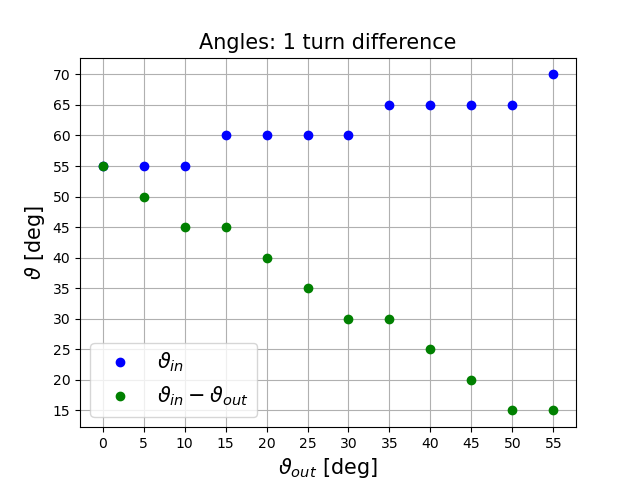
\includegraphics[width=0.49\textwidth, keepaspectratio]{Figures/muEDM/CyFi/Angles_1Turn_60deg_5deg.png}\label{fig:CyFi:5deg:angle}}
            \hfill
            \subfloat[Projected uncertainties as a function of the outer layer's angle]{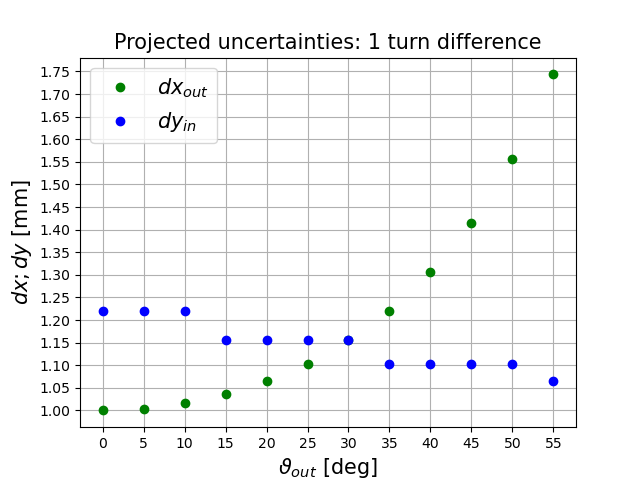
\includegraphics[width=0.49\textwidth, keepaspectratio]{Figures/muEDM/CyFi/projected_dxdy_1Turn_60deg_5deg.png}\label{fig:CyFi:5deg:projected_dxdy}}\\
            \subfloat[Fibers' length as a function of the outer layer's angle]{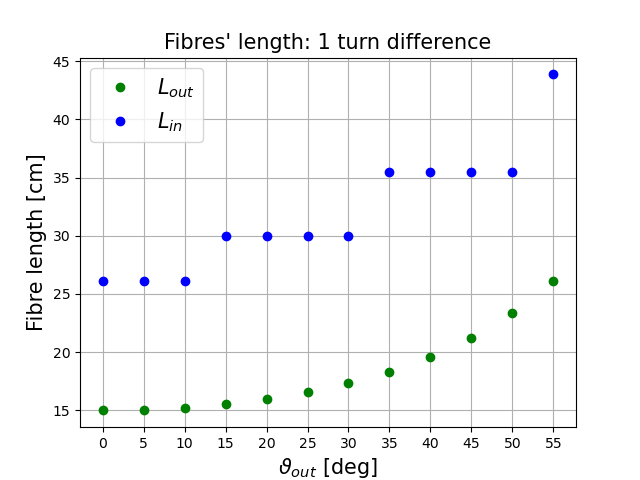
\includegraphics[width=0.49\textwidth, keepaspectratio]{Figures/muEDM/CyFi/FibreLength_1Turn_60deg_5deg.png}\label{fig:CyFi:5deg:length}}
            \caption[CHeT: key parameters with $\Delta T=1$ and 5 deg steps]{Key parameters as a function of the outer layer's angle keeping 1 turn difference between the two layers and rounding the angles to multiples of \SI{5}{\deg}.}
            \label{fig:CyFi:5deg}
        \end{figure}

    \status{done}
    \subsection{\gf simulation}
        The first hurdle in the Geant4 simulation for this sub-detector is the definition of the geometry.
        While the inside structure of the fibers and the readout are the same as discussed previously (see Sec.~\ref{sec:muEDM:fiber:g4}), the fiber shape is now less straightforward.
        
        \paragraph{G4TessellatedSolid}
        The shape is the result of wrapping a squared fiber around a cylinder resulting in a `squared helix'.
        After some consideration there are two ways of defying this geometry:
        \begin{outline}
            \1 Taking bool difference of two G4TwistedBox\footnote{The documentation can be found here: \href{https://apc.u-paris.fr/~franco/g4doxy/html/classG4TwistedBox.html}{\underline{G4TwistedBox}}}. 
            This is a simple solution but comes with some limitations: the shape of the fiber cannot be changed to circular and the twisted box cannot be twisted more than \SI{90}{\deg}, so a stack of clones is needed; 
            \1 Defying the geometry using G4TessellatedSolid\footnote{The documentation can be found here: \href{https://apc.u-paris.fr/~franco/g4doxy/html/classG4TessellatedSolid.html}{\underline{G4TessellatedSolid}}}, which means creating it by hand triangulating the shape. This is a more cumbersome solution but it allows for more flexibility.
        \end{outline}
        I decided to implement the latter to keep the possibility of simulating the detector with circular fibers.
        The core part of the code for generating the G4TessellatedSolid fibers, although perhaps not of particular interest, is in appendix \ref{ch:G4TessellatedSolid}.\\

        \noindent
        The resulting simulation, after having implemented everything so far described, is shown in Fig.~\ref{fig:CHeT:G4}, and is quite flexible: the dimensions of the CHeT, as well as the angles of the two layers and the fiber thickness, are parameters to be used when creating the CHeT geometry.

        \begin{figure}
            \centering
            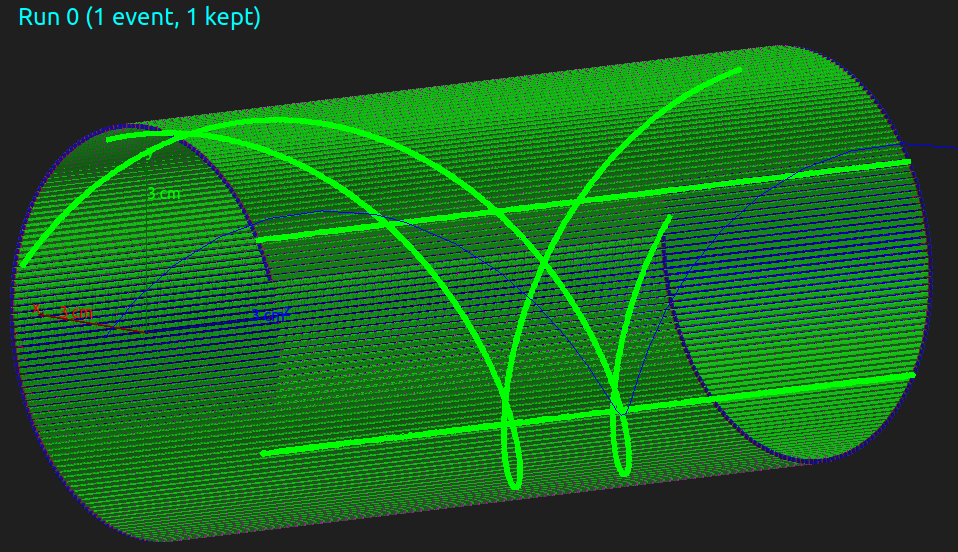
\includegraphics[width = 0.9\textwidth]{Figures/muEDM/CyFi/CHeT_G4.png}
            \caption[CHeT \gf: simulated event with two hits]{\gf simulation of the CHeT. The size of the fibers was increased to enhance the readability of the figure. While the structure may not be crystal clear, the fibers illuminated by the optical photons assist in guiding the eye along the two layers. In blue the particle traversing the detector.}
            \label{fig:CHeT:G4}
        \end{figure}
        
    \status{done}
    \subsection{From $\upgamma$s to waveforms}
        The simulation in \gf ends with the recording of the optical photons entering the SiPM SensitiveDetectors.
        The physical processes going from the impinging photons to the analog signal are quite complex and simulating them would require a lot of effort (and CPU time).
        To get a feeling of the type of signals we can expect from the simulation we can create a simple script \textit{faking} the readout.
        The required steps are:
        \begin{outline}
            \1 \textit{PDF}: probability of a photon converting. 
            This is a binomial distribution and is SiPM dependent: reasonable values $p_{PDF}\in [0.3, 0.5]$
            \1 \textit{Response}: per photon converted, add a 'waveform' at the photon time. 
            The shape $w(t)$ is SiPM/electronics dependent but some assumptions can be made.
            \1 \textit{Dead time}: when a pixel generates a signal, any additional photon coming within a $t_D$ is lost.
            \1 \textit{Dark noise}: add a probability of spurious photons converting. 
            This is a Poissonian process that gives $n_{dark}$ photons distributed flat in the readout time.
        \end{outline}
        \begin{equation}
            W(t)=\sum_{i=0}^{n_\gamma} w(t_i|\Delta t>t_D)\cdot p_{PDF} + \sum_{i=0}^{n_{dark}} w(t_{flat}) 
        \end{equation}
        Once we obtain $W(t)$ we can apply a threshold and turn the signal from analog to digital: when crossed, we recorded a \textit{hit}.
        In the geometry under consideration, a single particle crossing two fibers might generate 4 \textit{hits}, assuming reading the fibers at both ends.
        On top of this, the particle might generate scintillation in the neighbor fibers or some cross-talk might be present. 
        The general idea is to collect the signals from the fiber in each layer creating a 'layer'-\textit{hit} (a \textit{l-hit}). 
        This could then be combined to make a `cylinder'-\textit{hit} (a \textit{c-hit}).
        Mapping groups of hits in l/c-hits is not trivial and takes as parameters the dimensions of the cylinder and the SiPM numbers (or their position).

    \status{done}
    \subsection{Tracking}
    The details of the tracking procedure for the experiment are heavily dependent on the details of the detectors, which are not yet set in stone.
    The main options for a detector such as CHeT are:
    \begin{outline}
        \1 To combine the \textit{hits} from the two layers in \textit{c-hits}. This would result in smaller uncertainties in \textit{xyz} but requires delicate handling of the correlation between the variables plus reduces the number of available hits. This would also cut the number of hits in half
        \1 To consider the \textit{hits} separately still in \textit{xyz}
        \1 To perform a transformation for the \textit{hits} in a more `natural' coordinate system: $xyz\ra r\varphi z$
    \end{outline}

        \paragraph{GENFIT}
        The tracking code could be developed from scratch or based on pre-existing works. 
        Given the size of the collaboration and the task, the second solution seems more adequate.
        In this regard, a good option would be to rely on a code developed for general track fitting in particle physics is GENFIT\footnote{\href{https://github.com/GenFit/GenFit}{GENFIT: https://github.com/GenFit/GenFit}} \cite{GENFIT}\cite{GENFIT:2}.
        %A brief description of the code itself can be found in App.~\ref{ch:genfit}.
        The development of the tracking procedure for the CHeT detector had to be put to a halt. This section is kept here just as food for thought for future development.

        \paragraph{Ghost hits}
        Although requiring $\Delta T\leq1$ made so the same couple of fibers cannot cross multiple times, there is still a risk of ill-defined hits.
        If the particle hits the detector in two distinct places this will create a hit on 4 fibers. 
        If the timing resolution is not sufficient, this generates 4 possible interaction points.
        This situation is shown in Fig.~\ref{fig:CHeT:ghosts}, where the stars indicate the real hit locations.
        The existence of the other crossing point forces us to implement the double-end readout scheme.
        The resolution along the fiber will be enough to solve the redundancy of the ghost hits. 

    \begin{figure}
        \centering
        \subfloat[\gf simulation of the CHeT. An event to highlight the challenge of ghosts.]{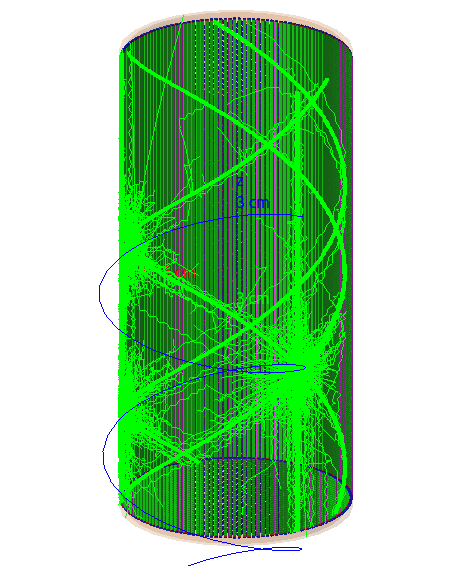
\includegraphics[width = 0.35\textwidth]{Figures/muEDM/CyFi/CHeT_G4_verty.png}\label{fig:CHeT:G4_verty}}\hfill
        \subfloat[Fibers from different `real' hits can still generate \textit{ghosts}. Marked with the star the `real hits' and with dots every crossing.]{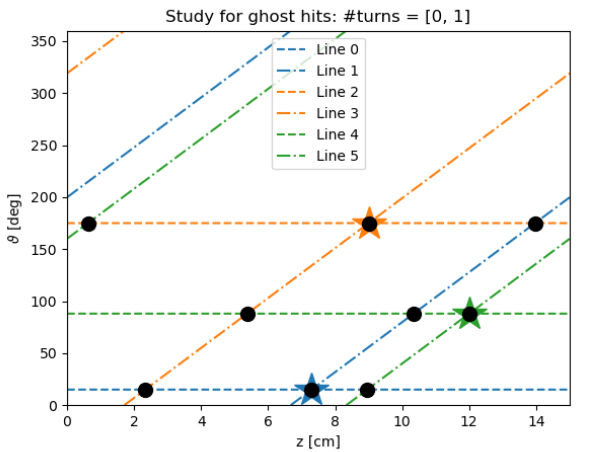
\includegraphics[width = 0.6\textwidth]{Figures/muEDM/CyFi/CHET_ghost_study.png}\label{fig:CHeT:ghosts}}
        \caption[ CHeT \gf: \textit{ghost} from different hits]{The $\Delta T\leq1$ requirement prevents fibers from crossing multiple times, but there is a risk of ambiguous hits. If a particle hits the detector in multiple places, with inadequate timing resolution, multiple potential interaction points arise, as illustrated in Fig.~\ref{fig:CHeT:ghosts}, with stars denoting real hits. To address this, we will implement a double-end readout scheme, with sufficient resolution to resolve ghost hits.}
        \label{fig:CHeT}
    \end{figure}

\status{done}
\section{A study of radial geometry}
    The development of the Pixel detector, supposed to be a counterpart to the CHeT, unfortunately, had some delay.
    This means that, during the first phase, the Pixel detector will not be available and the scintillating fibers need to be repurposed to be the only positron tracking detector.
    The designs discussed up until now do not collect enough hits to be the sole tracker, hence requiring going back to the drawing board.\\
    
    \noindent
    To rapidly study possible geometries, we opted for quick \gf simulations, in which the ribbons of fibers are approximated by solid scintillator volumes with no scintillation properties.
    This allows us to take into consideration the energy loss and multiple scattering the positron undergoes, saving the CPU time required to run an optical simulation, tracking each optical photon bouncing in the scintillator.\\

    \status{done}
    \subsection{Possible geometries}
        After a few iterations, the option of having a radial solution with crossed ribbons, as shown in Fig.~\ref{fig:eXSUN} was discarded. 
        Although crossed fibers improve the $\hat{y}$ resolution, as discussed in Sec.~\ref{sec:muEDM:CHeT:crossed}, it also increases the space required for the tracker at both ends, making the mechanics more complicated and adding material to the particle trajectory in non-interesting regions.\\

        \noindent
        The most promising solutions seem to be:
        \begin{outline}
            \1 A purely radial geometry (see Fig.~\ref{fig:eSUN}), with ribbons of longitudinal fibers alternated to (if needed shorter) ribbons of fibers running radially, delivering the good resolution on $\hat{y}$
            \1 A radial geometry of vertical fibers (with fewer ribbons) complemented by an internal barrel for the same reason, analogous to the inner part of the detector discussed in Sec.~\ref{sec:muEDM:proposal}.
        \end{outline}

        \begin{figure}
            \centering
            \subfloat[Crossed radial ribbons geometry.]{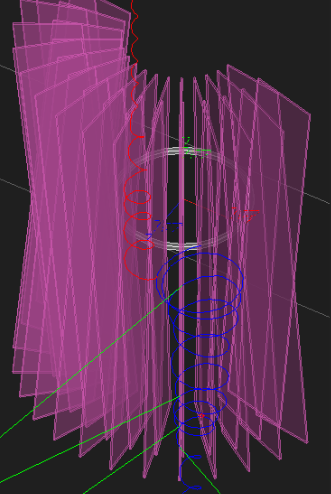
\includegraphics[height = 7.5cm]{Figures/muEDM/eTracker/eXSUN.png}\label{fig:eXSUN}}{}
            \subfloat[Simple radial geometry.]{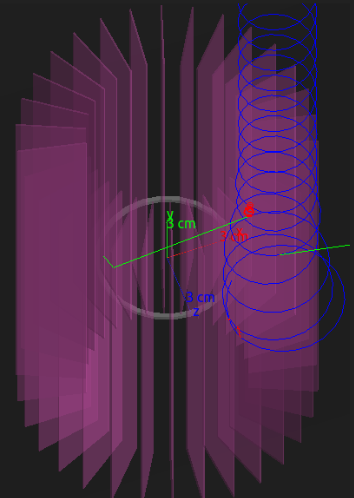
\includegraphics[height = 7.5cm]{Figures/muEDM/eTracker/eSUN.png}\label{fig:eSUN}}{}
        \caption[Additional radial geometries for the tracker]{Additional radial geometries are under study to overcome the absence of the pixel detector.} 
        \end{figure}
\status{done}
\section{Conclusions}
    This chapter describes the designs and simulations of the positron tracker.
    As of right now, some requirements for such a system are still `blurry'.
    Understanding the different aspects of the muEDM search generates requirements for the subsystem which are updated and, in turn, change the whole design of the experiment.
    The design included in the proposal nicely satisfied the requirements but presented some challenges in the readout, particularly for the inner barrel of the transverse layer.
    The `updated' CHeT design overcame the readout challenge at the cost of introducing a challenge due to the possible ambiguity of the hits (ghosts).
    Given the delay foreseen on the Pixel side, the requirements for the fiber sub-system changed.
    This prompted additional studies to develop different geometries that would be autonomous and self-sufficient in the positron tracking (at least for Phase I).
    
\status{done}
\printbibliography[
    heading = bibliographychapter,
    title=Bibliography on muEDM positron tracker
]

\end{refsection}